\documentclass[12pt,letterpaper,reqno]{article}

% \usepackage{mathtools}
\usepackage{epsfig}
\usepackage{amsmath}
\usepackage{amssymb}
\usepackage{amsthm}
\usepackage{indentfirst}
\usepackage{xspace}
\usepackage{multirow}
\usepackage{hyperref}
\usepackage{xcolor}
\usepackage{verbatim}
\usepackage[letterpaper,margin=1in,headheight=15pt]{geometry}
\usepackage{mathpazo}
\usepackage{tikz-cd}
\usepackage{booktabs}
\usepackage{framed}
\usepackage{float}
\usepackage{thmtools}
\usepackage{dashrule}
\usepackage[missing=]{gitinfo2}
\usepackage{fancyhdr}
\usepackage{enumerate}
\usepackage{graphicx}
\usepackage{mathrsfs}
\usepackage{calligra}
\usepackage[titletoc,title]{appendix}
\usepackage{caption}
\usepackage{subcaption}

\definecolor{darkblue}{rgb}{0.1,0.1,0.7}
\definecolor{darkred}{rgb}{0.5,0.1,0.1}
\definecolor{darkgreen}{rgb}{0.0,0.42,0.06}
\hypersetup{colorlinks=true,urlcolor=darkred,linkcolor=darkblue,citecolor=darkred}
\definecolor{shadecolor}{rgb}{0.85,0.85,0.85}

% Bibliography formatting
\usepackage[bibstyle=authoryear-comp,labeldate=false,defernumbers=true,maxnames=20,uniquename=init,dashed=false,backend=biber,sorting=none]{biblatex}

\DeclareNameAlias{sortname}{first-last}

\DeclareFieldFormat{url}{\url{#1}}
\DeclareFieldFormat[article]{pages}{#1}
\DeclareFieldFormat[inproceedings]{pages}{\lowercase{pp.}#1}
\DeclareFieldFormat[incollection]{pages}{\lowercase{pp.}#1}
\DeclareFieldFormat[article]{volume}{\textbf{#1}}
\DeclareFieldFormat[article]{number}{(#1)}
\DeclareFieldFormat[article]{title}{\MakeCapital{#1}}
\DeclareFieldFormat[inproceedings]{title}{#1}
\DeclareFieldFormat{shorthandwidth}{#1}

% Don't use "In:" in bibliography. Omit urls from journal articles.
\DeclareBibliographyDriver{article}{%
  \usebibmacro{bibindex}%
  \usebibmacro{begentry}%
  \usebibmacro{author/editor}%
  \setunit{\labelnamepunct}\newblock
  \MakeSentenceCase{\usebibmacro{title}}%
  \newunit
  \printlist{language}%
  \newunit\newblock
  \usebibmacro{byauthor}%
  \newunit\newblock
  \usebibmacro{byeditor+others}%
  \newunit\newblock
  \printfield{version}%
  \newunit\newblock
%  \usebibmacro{in:}%
  \usebibmacro{journal+issuetitle}%
  \newunit\newblock
  \printfield{note}%
  \setunit{\bibpagespunct}%
  \printfield{pages}
  \newunit\newblock
  \usebibmacro{eprint}
  \newunit\newblock
  \printfield{addendum}%
  \newunit\newblock
  \usebibmacro{pageref}%
  \usebibmacro{finentry}}

% Remove dot between volume and number in journal articles.
\renewbibmacro*{journal+issuetitle}{%
  \usebibmacro{journal}%
  \setunit*{\addspace}%
  \iffieldundef{series}
    {}
    {\newunit
     \printfield{series}%
     \setunit{\addspace}}%
  \printfield{volume}%
%  \setunit*{\adddot}%
  \printfield{number}%
  \setunit{\addcomma\space}%
  \printfield{eid}%
  \setunit{\addspace}%
  \usebibmacro{issue+date}%
  \newunit\newblock
  \usebibmacro{issue}%
  \newunit}


% Bibliography categories
\def\makebibcategory#1#2{\DeclareBibliographyCategory{#1}\defbibheading{#1}{\section*{#2}}}
\makebibcategory{books}{Books}
\makebibcategory{papers}{Refereed research papers}
\makebibcategory{chapters}{Book chapters}
\makebibcategory{conferences}{Papers in conference proceedings}
\makebibcategory{techreports}{Unpublished working papers}
\makebibcategory{bookreviews}{Book reviews}
\makebibcategory{editorials}{Editorials}
\makebibcategory{phd}{PhD thesis}
\makebibcategory{subpapers}{Submitted papers}
\makebibcategory{curpapers}{Current projects}

\setlength{\bibitemsep}{2.65pt}
\setlength{\bibhang}{.8cm}
\renewcommand{\bibfont}{\small}

\renewcommand*{\bibitem}{\addtocounter{papers}{1}\item \mbox{}\hskip-0.85cm\hbox to 0.85cm{\hfill\arabic{papers}.~~}}
\defbibenvironment{bibliography}
{\list{}
  {\setlength{\leftmargin}{\bibhang}%
   \setlength{\itemsep}{\bibitemsep}%
   \setlength{\parsep}{\bibparsep}}}
{\endlist}
{\bibitem}

\newenvironment{publications}{\section{\LARGE Publications}\label{papersstart}\vspace*{0.2cm}\small
\titlespacing{\section}{0pt}{1.5ex}{1ex}\itemsep=0.00cm
}{\label{papersend}\addtocounter{sumpapers}{-1}\refstepcounter{sumpapers}\label{sumpapers}}

\def\printbib#1{\printbibliography[category=#1,heading=#1]\lastref{sumpapers}}

% Counters for keeping track of papers
\newcounter{papers}\setcounter{papers}{0}
\newcounter{sumpapers}\setcounter{sumpapers}{0}
\def\lastref#1{\addtocounter{#1}{\value{papers}}\setcounter{papers}{0}}

% theorem environments
\declaretheoremstyle[spaceabove=0.25cm,spacebelow=0.25cm,notefont=\normalfont\bfseries, notebraces={(}{)}]{theorem}
\declaretheoremstyle[spaceabove=0.25cm,spacebelow=0.25cm,bodyfont=\normalfont,notefont=\normalfont\bfseries, notebraces={(}{)}]{noital}
\declaretheoremstyle[spaceabove=0.25cm,spacebelow=0.25cm,bodyfont=\normalfont\color{darkgreen},notefont=\normalfont\bfseries, notebraces={(}{)}]{green}
\declaretheoremstyle[spaceabove=0.25cm,spacebelow=0.25cm,bodyfont=\normalfont,notefont=\normalfont\bfseries,qed=$\qedsymbol$,notebraces={(}{)}]{proofstyle}

\declaretheorem[name=Theorem,numberwithin=section,style=theorem]{thm}
\declaretheorem[name=Proposition,sibling=thm,style=theorem]{prop}
\declaretheorem[name=Corollary,sibling=thm,style=theorem]{cor}
\declaretheorem[name=Lemma,sibling=thm,style=theorem]{lem}
\declaretheorem[name=Definition,sibling=thm,style=noital]{defn}
\declaretheorem[name=Example,sibling=thm,style=noital]{example}
\declaretheorem[name=Exercise,numberwithin=section,style=green]{exercise}
\declaretheorem[name=Proof,style=proofstyle,numbered=no]{pf}
\declaretheorem[name=Solution,style=proofstyle,numbered=no]{solution}
\declaretheorem[name=Remark,style=proofstyle,numbered=no]{remark}
\declaretheorem[name=Remarks,style=proofstyle,numbered=no]{remarks}
\numberwithin{equation}{section}


% macros for convenience
\newcommand{\tops}{\texorpdfstring}

\newcommand{\nid}{\noindent}

\newcommand{\fa}{{\mathfrak a}}
\newcommand{\fp}{{\mathfrak p}}
\newcommand{\fk}{{\mathfrak k}}
\newcommand{\fg}{{\mathfrak g}}
\newcommand{\fh}{{\mathfrak h}}
\newcommand{\fn}{{\mathfrak n}}
\newcommand{\fq}{{\mathfrak q}}
\newcommand{\fm}{{\mathfrak m}}
\newcommand{\fr}{{\mathfrak r}}
\newcommand{\fu}{{\mathfrak u}}
\newcommand{\fG}{{\mathfrak G}}

\newcommand{\cC}{\ensuremath{\mathcal C}}
\newcommand{\cG}{\ensuremath{\mathcal G}}
\newcommand{\cB}{\ensuremath{\mathcal B}}
\newcommand{\cL}{\ensuremath{\mathcal L}}
\newcommand{\cS}{\ensuremath{\mathcal S}}
\newcommand{\cF}{\ensuremath{\mathcal F}}
\newcommand{\cK}{\ensuremath{\mathcal K}}
\newcommand{\cZ}{\ensuremath{\mathcal Z}}
\newcommand{\cM}{\ensuremath{\mathcal M}}
\newcommand{\cN}{\ensuremath{\mathcal N}}
\newcommand{\cO}{\ensuremath{\mathcal O}}
\newcommand{\cH}{\ensuremath{\mathcal H}}
\newcommand{\cX}{\ensuremath{\mathcal X}}
\newcommand{\cY}{\ensuremath{\mathcal Y}}
\newcommand{\cA}{\ensuremath{\mathcal A}}
\newcommand{\cI}{\ensuremath{\mathcal I}}

\newcommand{\R}{\ensuremath{\mathbb R}}
\newcommand{\C}{\ensuremath{\mathbb C}}
\newcommand{\PP}{\ensuremath{\mathbb P}}
\newcommand{\Z}{\ensuremath{\mathbb Z}}
\newcommand{\Q}{\ensuremath{\mathbb Q}}
\newcommand{\A}{\ensuremath{\mathbb A}}
\newcommand{\bbH}{\ensuremath{\mathbb H}}
\newcommand{\bbI}{\ensuremath{\mathbb I}}
\newcommand{\bS}{\ensuremath{\mathbb S}}

\newcommand{\half}{\ensuremath{\frac{1}{2}}}
\newcommand{\qtr}{\ensuremath{\frac{1}{4}}}
\newcommand{\bq}{{\mathbf q}}
\newcommand{\N}{{\mathcal N}}
\newcommand{\F}{{\mathcal F}}
\newcommand{\HH}{{\mathcal H}}
\newcommand{\LL}{{\mathcal L}}
\newcommand{\RR}{{\mathcal R}}
\newcommand{\V}{{\mathcal V}}
\newcommand{\dirac}{\!\!\not\!\partial}
\newcommand{\Dirac}{\!\!\not\!\!D}
\newcommand{\cE}{{\mathcal E}}
\newcommand{\vs}{\not\!v}
\newcommand{\kahler}{K\"ahler\xspace}
\newcommand{\kq}{/\!\!/}
\newcommand{\kql}[1]{/\!\!/\!\!_#1\,}
\newcommand{\hk}{hyperk\"ahler\xspace}
\newcommand{\Hk}{Hyperk\"ahler\xspace}
\newcommand{\hkq}{/\!\!/\!\!/\!\!/}
\newcommand{\hkql}[1]{/\!\!/\!\!/\!\!/\!\!_#1\,}
\newcommand{\del}{\ensuremath{\partial}}
\newcommand{\delbar}{\ensuremath{\overline{\partial}}}
\newcommand{\bl}{{\bf L}}
\newcommand{\J}{{\mathrm j}}
\newcommand{\K}{{\mathrm k}}
\newcommand{\e}{{\mathrm e}}
\newcommand\bid{{\mathbf 1}}
\newcommand{\de}{\mathrm{d}}
\newcommand{\ab}{\mathrm{ab}}
\newcommand{\vol}{\mathrm{vol}}
\renewcommand{\sf}{\mathrm{sf}}
\newcommand{\inst}{\mathrm{inst}}
\newcommand{\eff}{\mathrm{eff}}
\newcommand{\dR}{\mathrm{dR}}
\newcommand{\closed}{\mathrm{closed}}
\newcommand{\exact}{\mathrm{exact}}

\newcommand{\abs}[1]{\lvert#1\rvert}
\newcommand{\norm}[1]{\lVert#1\rVert}
\newcommand{\IP}[1]{\langle#1\rangle}
\newcommand{\DIP}[1]{\langle\!\langle#1\rangle\!\rangle}
\newcommand{\dwrt}[1]{\frac{\partial}{\partial#1}}
\newcommand{\eps}{\epsilon}
\newcommand{\simarrow}{\xrightarrow\sim}

\newcommand{\mmaref}[1]{}

\newcommand{\ti}[1]{\textit{#1}}
\newcommand{\tb}[1]{\textbf{#1}}
\newcommand{\lo}{\text{\calligra o}\,}
\newcommand{\dd}{\ensuremath{\mathscr{D}}}
\newcommand{\bu}{{\bf u}}
\newcommand{\bv}{{\bf v}}
\newcommand{\bw}{{\bf w}}
\newcommand{\bx}{{\bf x}}
\newcommand{\by}{{\bf y}}
\newcommand{\bz}{{\bf z}}
\newcommand{\ba}{{\bf a}}
\newcommand{\bb}{{\bf b}}
\newcommand{\bbr}{{\bf r}}
\newcommand{\bff}{{\bf f}}
\newcommand{\bgg}{{\bf g}}
\newcommand{\bt}{{\bf t}}
\newcommand{\bn}{{\bf n}}
\newcommand{\ii}{{\bf {\hat{i}}}}
\newcommand{\jj}{{\bf {\hat{j}}}}
\newcommand{\kk}{{\bf {\hat{k}}}}
\newcommand{\ut}{{\bf {\hat{t}}}}
\newcommand{\un}{{\bf {\hat{n}}}}
\newcommand{\ub}{{\bf {\hat{b}}}}


\DeclareMathOperator{\ad}{ad}
\DeclareMathOperator{\im}{Im}
\DeclareMathOperator{\re}{Re}
\DeclareMathOperator{\Tr}{Tr}
\DeclareMathOperator{\End}{End}
\DeclareMathOperator{\Hom}{Hom}
\DeclareMathOperator{\Aut}{Aut}
\DeclareMathOperator{\Sym}{Sym}
\DeclareMathOperator{\Lie}{Lie}
\DeclareMathOperator{\diag}{diag}
\DeclareMathOperator{\Bun}{Bun}
\DeclareMathOperator{\Vect}{Vect}
\DeclareMathOperator{\Span}{Span}
\DeclareMathOperator{\grad}{grad}
\DeclareMathOperator{\rank}{rank}
\DeclareMathOperator{\ind}{ind}
\DeclareMathOperator{\coker}{coker}
\DeclareMathOperator{\Jac}{Jac}
\DeclareMathOperator{\Hol}{Hol}
\DeclareMathOperator{\gr}{gr}

\newcommand{\insfig}[2]{

\medskip
\noindent
\begin{minipage}{\linewidth}

\makebox[\linewidth]{\includegraphics[keepaspectratio=true,scale=#2]{figures/#1-crop.pdf}}

\end{minipage}
\medskip

}


% \newcommand{\insfig}[2]{\begin{figure}[htbp] \centering \includegraphics[scale=#2]{figures/#1-crop.pdf} \label{fig:#1} \end{figure}}
% syntax: \insfig{name}{0.5}{caption}

\newcommand{\fixme}[1]{{\color{orange}{[#1]}}}
\newcommand{\currentposition}{{\color{blue} \noindent\makebox[\linewidth]{\hdashrule{\paperwidth}{1pt}{3mm}}}}

% \mathtoolsset{showonlyrefs}

\bibliography{mvc}

\begin{document}
\pagestyle{fancy}
\lhead{{\tiny \color{gray} \tt \gitAuthorIsoDate}}
\chead{\tiny \ti{Multivariable Calculus, GSMST Spring 2020}}
\rhead{{\tiny \color{gray} \tt \gitAbbrevHash}}
\renewcommand{\headrulewidth}{0.5pt}


\begin{center}
\tb{Multivariable Calculus} \\
Anderson Trimm \\
Gwinnett School of Mathematics, Science and Technology \\
\end{center}

{These are the notes for the Spring Semester 2020
course in Multivariable Calculus at GSMST. They will continually be updated throughout the course. The latest PDF can always be accessed
at \small \url{https://github.com/atrimm/mvc/blob/master/Course%20Notes/multivariable_calculus_2020.pdf.}

\tableofcontents
\renewcommand{\listtheoremname}{Quick reference}
\listoftheorems[onlynamed]

\newpage

%\setcounter{page}{1}

\section{Curves}
In this section we study functions with one input and multiple outputs.

\subsection{Vector-valued functions}
\subsubsection{Definitions}
Suppose a particle moves in the plane along the following curve $C$:
	\begin{center}
		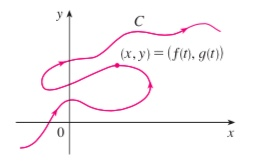
\includegraphics[scale=0.5]{figures_mvc/plane_curve}
	\end{center}
Since the curve fails the vertical line test, $C$ cannot be described as the graph of a function $y=f(x)$. Note however that the x- and y-coords of the particle are functions of time
\begin{align*}
	x=f(t), \hspace{0.5cm} y=g(t)
\end{align*}
so the curve $C$ can be described as the image of function ${\bf r}:I \to \mathbb{R}^2$ defined by 
\begin{align*}
	\bbr(t)=(f(t),g(t)),
\end{align*}
where $I=[a,b]$ is an interval in $\R$. \fixme{Add mapping diagram.}

\begin{defn}[Vector-valued function]
Let $U \subseteq \R$. A mapping $\bbr:U \to \mathbb{R}^n$ called a \emph{vector-valued function}. The value of $\bbr$ at $t \in U$ can be written as
\begin{align*}
	\bbr(t)=(r_1(t),r_2(t),\dots,r_n(t))
\end{align*}
where the $n$ functions $r_i:U \to \R$, $i=1,\dots,n$ are called the \emph{component functions} of $\bbr$.	
\end{defn}
Unless specified otherwise, we will take the domain $U$ of a vector-valued function to be the largest domain on which all of the component functions are defined.
\begin{example}
Consider the vector-valued function $\bbr:U \to \mathbb{R}^3$ defined by
	\begin{align*}
		\bbr(t)=(t^3,\ln(3-t),\sqrt{t}).
	\end{align*}
The component functions of $\bbr(t)$ are 
\begin{align*}
	r_1(t)=t^3, \hspace{0.5cm} r_2(t)=\ln(3-t), \hspace{0.5cm} r_3(t)=\sqrt{t}.
\end{align*}
The domains of each of these functions, respectively, are 
\begin{align*}
	U_1=\R, \hspace{0.5cm} U_2=(-\infty,3), \hspace{0.5cm} U_3=[0,\infty),
\end{align*}	
so the domain $U$ of $\bbr(t)$ is 
\begin{align*}
	U=U_1 \cap U_2 \cap U_3=[0,3).
\end{align*} 
\end{example}

\begin{exercise}
	Consider the vector-valued function $\bbr:U \to \mathbb{R}^3$ defined by
	\begin{align*}
		\bbr(t)=\left(\frac{t-2}{t+2},\sin t, \ln(9-t^2)\right).
	\end{align*}
What is the domain $U$ of the function?
\end{exercise}
{\color{red}\begin{solution}
	The component functions of $\bbr(t)$ are 
	\begin{align*}
		r_1=\frac{t-2}{t+2}, \hspace{0.5cm} r_2=\sin t, \hspace{0.5cm} r_3=\ln(9-t^2).
	\end{align*}
	The domains of $r_1(t)$ and $r_2(t)$ are given, respectively, by
	\begin{align*}
		U_1=(-\infty,2) \cup (2,\infty), \hspace{0.5cm} U_2=\R.
	\end{align*}
	To find the domain of $r_3(t)$, we need to solve the inequality
	\begin{align*}
		9-t^2>0. \\
	\end{align*}
	The graph of the function $y=9-x^2$ is a concave-down parabola with $y$-intercept 9 and $x$-intercepts $\pm 3$. 
	
	\begin{figure}[h]
	\begin{center}
		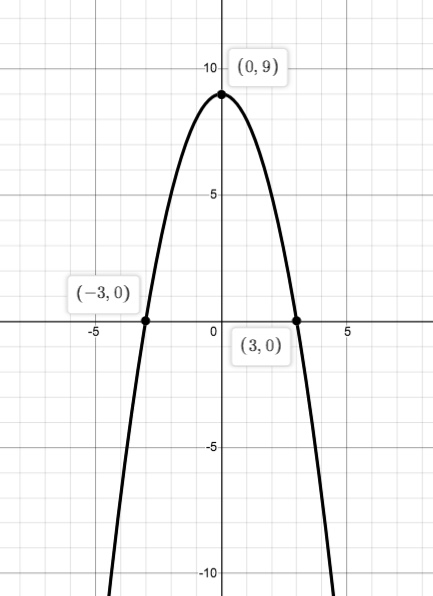
\includegraphics[scale=0.3]{figures_mvc/parab_down}
	\end{center}
	\caption{Graph of $y=9-x^2$.}
\end{figure}
	We have $y>0$ where the graph is above the $x$-axis, so $y>0$ when $-3<x<3$. The domain of $r_3(t)$ is therefore
	\begin{align*}
		U_3=(-3,3).
	\end{align*}
	The domain of $\bbr(t)$ is then
	\begin{align*}
		U=U_1 \cap U_2 \cap U_3=(-3,-2)\cup (-2,3).
	\end{align*}
\end{solution}}

\subsubsection{Review: limits of single-variable functions}
Before considering limits of vector-valued functions, let's review the definition for a real-valued function $y=f(x)$ of a single real variable $x$.

To motivate the definition, consider the function
\begin{align*}
	f(x)=\begin{cases}
		2x-1, \ \text{ if } x \neq 3 \\
		6, \hspace{1.0cm} \text{ if } x = 3 \\
	\end{cases}
\end{align*}
whose graph is shown in the figure below.

\begin{figure}[h]\label{fig:lim_def}
	\begin{center}
		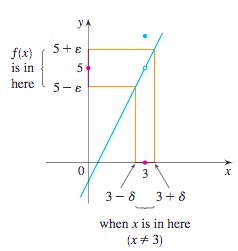
\includegraphics[scale=0.7]{figures_mvc/graph_limit_defn}
	\end{center}
	\caption{Graph of the function $y=f(x)$ in the example above.}
\end{figure}
From the graph, we see that when $x$ is close to 3 but not equal to 3, then $f(x)$ is close to 5, and so $\lim_{x \to 3}f(x)=5$.

To obtain more detailed information about how $f(x)$ varies when $x$ is close to 3, we ask the following question: 

\emph{How close to 3 does $x$ have to be so that $f(x)$ differs from 5 by less than $0.1$?}

The distance from $x$ to $3$ is $|x-3|$ and the distance from $f(x)$ to 5 is $|f(x)-5|$, so our problem is to find a number $\delta$ such that 
\begin{align*}
	|f(x)-5|<0.1 \hspace{0.5cm} \text{ if } \hspace{0.5cm} 0<|x-3|<\delta.
\end{align*}
If $x \neq 3$, then 
\begin{align*}
	|f(x)-5|=|(2x-1)-5|=|2x-6|=2|x-3|
\end{align*}
so we see that by taking $\delta=\frac{1}{2}(0.1)=0.05$, we have $|f(x)-5|<2(0.05)=0.1$. Thus, an answer to the problem is given by $\delta=0.05$; that is, if $x$ is within a distance of $0.05$ from 3, then $f(x)$ will be within a distance of $0.1$ from 5.

If we change the number $0.1$ in our problem to the smaller number $0.01$, then by using the same method we find that $f(x)$ will differ from 5 by less than $0.01$ provided that $x$ differs from 3 by less than $\frac{1}{2}(0.01)=0.005$; that is,
\begin{align*}
	|f(x)-5|<0.01 \hspace{0.5cm} \text{ if } \hspace{0.5cm} 0<|x-3|<0.005.
\end{align*}
Similarly,
\begin{align*}
	|f(x)-5|<0.001 \hspace{0.5cm} \text{ if } \hspace{0.5cm} 0<|x-3|<0.0005.
\end{align*}
Think of the numbers $0.1, 0.01, 0.001$ above as \emph{error tolerances} that we might allow. That is, when challenged with an error tolerance, it is our task to find a corresponding $\delta$ so that whenever $x$ is within a distance of $\delta$ from 3, $f(x)\approx 5$, within the given error tolerance. 

Now for 5 to be the precise limit of $f(x)$ as $x$ approaches 3, we must not only be able to bring the difference between $f(x)$ and 5 below each of these numbers; we must be able to bring it below \emph{any} positive number. And, by exactly the same reasoning, we can. That is, if $\epsilon$ is any positive number, then by choosing $\delta=\frac{\epsilon
}{2}$, we find
\begin{align}\label{eq:review_limit_example}
	|f(x)-5|<\epsilon \hspace{0.5cm} \text{ if } \hspace{0.5cm} 0<|x-3|<\delta=\frac{\epsilon}{2}.
\end{align}
This is a precise way of saying that $f(x)$ is close to 5 when $x$ is close to 3, because Equation \eqref{eq:review_limit_example} says that we can make the values of $f(x)$ within an arbitrary distance $\epsilon$ from 5 by taking the values of $x$ within a distance $\frac{\epsilon}{2}$ from 3 (but $x \neq 3$).

Note that Equation \eqref{eq:review_limit_example} can be rewritten as follows:
\begin{align*}
	\text{ if } \hspace{0.5cm} 3-\delta<x<3+\delta \hspace{0.2cm} (x \neq 3) \hspace{0.5cm} \text{ then } \hspace{0.5cm} 5-\epsilon<f(x)<5+\epsilon
\end{align*}
as illustrated in the figure above. This says that by taking the values of $x$ ($x \neq 3$) to lie in the interval $(3-\delta,3+\delta)$ we can make the values of $f(x)$ lie in the interval $(5-\epsilon,5+\epsilon)$.

Following the reasoning in this example,  the precise definition of a limit is the following.

\begin{defn}[Limit of a single-variable function]\label{def:limit_of_a_single-variable_function}
	Let $(a,b)$ be an open interval containing the point $x_0$ and let $f(x)$ be a real-valued function defined on this interval, except possibly at $x_0$ itself. A number $L$ is called the \emph{limit of $f(x)$ as $x$ approaches $x_0$} if for every $\epsilon>0$ there exists a $\delta>0$ such that $|f(x)-L|<\epsilon$ whenever $0<|x-x_0|<\delta$. If such an $L$ exists, we write
	\begin{align*}
		\lim_{x \to x_0}f(x)=L.
	\end{align*}
\end{defn}

\begin{thm}[Uniqueness of limits]\label{thm:uniqueness_of_limits}
	If $f(x)$ has a limit $L$ at $x_0$, then the limit is unique.
\end{thm}

\begin{pf}
Suppose that $\lim_{x \to x_0}f(x)=L$ and $\lim_{x \to x_0}f(x)=L'$. Then, given any $\epsilon>0$ there exist positive numbers $\delta_1$ and $\delta_2$ such that 
\begin{align*}
	|f(x)-L|<\frac{\epsilon}{2} \hspace{0.5cm} \text{ if } \hspace{0.5cm} |x-x_0|<\delta_1
\end{align*} 	
and
\begin{align*}
	|f(x)-L'|<\frac{\epsilon}{2} \hspace{0.5cm} \text{ if } \hspace{0.5cm} |x-x_0|<\delta_2.
\end{align*} 
Then by taking $|x-x_0|<\delta=\min\{\delta_1,\delta_2\}$, we have
\begin{align*}
	|L-L'|=|L-L'+f(x)-f(x)|=|L-f(x)+f(x)-L|\leq |f(x)-L|+|f(x)-L'|<\frac{\epsilon}{2}+\frac{\epsilon}{2}=\epsilon.
\end{align*}
For this to be true for all $\epsilon>0$, we must have $L-L'=0$, or $L=L'$.
\end{pf}


\begin{exercise}
Use Definition \ref{def:limit_of_a_single-variable_function} to prove that $\lim_{x \to 3}(4x-5)=7$.
\end{exercise}

{\color{red} \begin{solution}
Let $\epsilon>0$. For all $x \neq 3$, 
\begin{align*}
	|f(x)-7|=|(4x-5)-7|=|4x-12|=4|x-3|.
\end{align*} 
By taking $\delta=\frac{\epsilon}{4}$, we have $0<|x-3|<\frac{\epsilon}{4}$ and therefore
\begin{align*}
	|f(x)-7|=4|x-3|<4\cdot \frac{\epsilon}{4}=\epsilon,
\end{align*}	
which proves that $\lim_{x \to 3}(4x-5)=7$.
\end{solution}}

\begin{example}
We now use Definition \ref{def:limit_of_a_single-variable_function} to prove that $\lim_{x \to 3}x^2=9$.	

Let $\epsilon>0$. For all $x \neq 3$, we have
\begin{align*}
	|f(x)-9|=|x^2-9|=|(x+3)(x-3)|=|x+3||x-3|.
\end{align*} 
Notice that if we can find a positive number $C$ such that $|x+3|<C$, then
\begin{align*}
	|x+3||x-3|<C|x-3|
\end{align*}
and we can make $C|x-3|<\epsilon$ by taking $|x-3|<\frac{\epsilon}{C}=\delta$. We can find such a number $C$ if we restrict $x$ to lie in some interval centered at 3. Since we are only interested in values of $x$ that are close to 3, this is exactly what we want. Let's assume that $|x-3|<\alpha$ for some positive number $\alpha$, say $\alpha=1$ (it does not matter what number we take here). Then we have
\begin{align*}
	x-3<1 \hspace{0.5cm} \text{ or }  \hspace{0.5cm} -x+3<1.
\end{align*}
The first inequality says $x<4$ and the second says $2<x$, so $|x-3|<1$ implies that 
\begin{align*}
	2<x<4.
\end{align*}
Adding 3 to both sides of this inequality gives 
\begin{align*}
	5<x+3<7,
\end{align*}
and therefore $|x+3|<|7|=7=C$. But now there are two restrictions on $|x-3|$, namely
\begin{align*}
	|x-3|<1 \hspace{0.5cm} \text{ and } \hspace{0.5cm} |x-3|<\frac{\epsilon}{C}=\frac{\epsilon}{7}.
\end{align*}
To make sure that both of these inequalities are satisfied, we take $\delta=\min\{1,\frac{\epsilon}{7}\}$. Since $0<|x-3|<\delta$ implies $|x^2-9|<\epsilon$, this proves that $\lim_{x \to 3}x^2=9$.
\end{example}
The previous example shows that it is not always easy to prove that a function has a particular limit using Definition \ref{def:limit_of_a_single-variable_function}. In fact, if we had considered a more complicated function such as 
\begin{align*}
	f(x)=\frac{6x^2-8x+9}{2x^2-1}
\end{align*}
then proving that $\lim_{x \to 1}f(x)=7$ using Definition \ref{def:limit_of_a_single-variable_function} would require a great deal of ingenuity. Instead, we prove the following theorems, which makes evaluating limits much easier.

\begin{lem}[Triangle Inequality]\label{lem:triangle_inequality}
	For all $x,y \in \R$, 
	\begin{align*}
		|x+y| \leq |x|+|y|.
	\end{align*}
\end{lem}

\begin{pf}
We have
\begin{align*}
	|x+y|^2=(x+y)^2&=x^2+y^2+2xy \\
	&=|x|^2+|y|^2+2xy \\
	&\leq |x|^2+|y|^2+2|x||y| \\
	&=(|x|+|y|)^2.
\end{align*}	
Since both sides are nonnegative, this implies that 
\begin{align*}
	|x+y| \leq |x|+|y|.
\end{align*}
\end{pf}



\begin{thm}[Limit laws for single-variable functions]\label{thm:limit_laws_for_single-variable_functions}
Suppose $f(x)$ and $g(x)$ are defined on the same open set containing $x_0$, and that 
\begin{align*}
	\lim_{x \to x_0}f(x)=L \hspace{0.5cm} \text{ and } \hspace{0.5cm} \lim_{x \to x_0}g(x)=M.
\end{align*}
Then
	\begin{enumerate}[(i)]
		\item $\lim_{x \to x_0}c=c$ for any constant $c \in \R$.
		\item $\lim_{x \to x_0}x=x_0$.
		\item $\lim_{x \to x_0} cf(x)=cL$ for any $c \in \R$;
		\item $\lim_{x \to x_0}(f(x)+ g(x))=L+M$;
		\item $\lim_{x \to x_0}(f(x)g(x))=LM$;
		\item $\lim_{x \to x_0}=\frac{f(x)}{g(x)}=\frac{L}{M}$ whenever $M \neq 0$.
	\end{enumerate}
\end{thm}

\begin{pf}
\begin{enumerate}[(i)]
	\item Let $\epsilon>0$. Since $|c-c|=0$, $|c-c|<\epsilon$ whenever $|x-x_0|<\delta$ for any positive number $\delta$.
	\item Given $\epsilon>0$, by taking $\delta=\epsilon$ we have $|x-x_0|<\epsilon$ whenever $|x-x_0|<\delta=\epsilon$.
	\item Since $\lim_{x \to x_0}f(x)=L$, given $\epsilon>0$ there exists a corresponding $\delta>0$ such that $|f(x)-L|<\epsilon$ whenever $0<|x-x_0|<\delta$. Then $|cf(x)-cL|=|c||f(x)-L|<\epsilon$ whenever $0<|x-x_0|<\frac{\epsilon}{|c|}$.
	\item We have
	\begin{align*}
		|f(x)+g(x)-(L+M)|=|(f(x)-L)+(g(x)-M)| \leq |f(x)-L|+|g(x)-M|
	\end{align*}
	by the Triangle Inequality (Lemma \ref{lem:triangle_inequality}). Since $\lim_{x \to x_0}f(x)=L$ and $\lim_{x \to x_0}g(x)=M$, given $\epsilon>0$ there exist positive numbers $\delta_1$ and $\delta_2$ such that 
	\begin{align*}
		|f(x)-L|<\frac{\epsilon}{2} \hspace{0.5cm} \text{ if } \hspace{0.5cm} |x-x_0|<\delta_1
	\end{align*} 
	and 
	\begin{align*}
		|g(x)-M|<\frac{\epsilon}{2} \hspace{0.5cm} \text{ if } \hspace{0.5cm} |x-x_0|<\delta_2.
	\end{align*} 
	By taking $|x-x_0|<\delta=\min\{\delta_1,\delta_2\}$, we have 
	\begin{align*}
		|f(x)+g(x)-(L+M)|\leq |f(x)-L|+|g(x)-M|<\frac{\epsilon}{2}+\frac{\epsilon}{2}=\epsilon,
	\end{align*}
	which proves that $\lim_{x \to x_0}(f(x)+g(x))=L+M$.
	\item First, note that
		\begin{align*}
			f(x)g(x)-LM&=(f(x)-L)(g(x)-M)+L(g(x)-M)+M(f(x)-L).
		\end{align*} 
		Let $\epsilon>0$. Since $\lim_{x \to x_0}f(x)=L$ there exists $\delta_1>0$ such that $|f(x)-L|<\sqrt{\epsilon}$ whenever $|x-x_0|<\delta_1$. Since $\lim_{x \to x_0}g(x)=M$ there exists $\delta_2>0$ such that $|g(x)-M|<\sqrt{\epsilon}$ whenever $|x-x_0|<\delta_2$. Then, whenever $|x-x_0|<\delta=\min\{\delta_1,\delta_2\}$, we have
		\begin{align*}
			|(f(x)-L)(g(x)-M)|=|f(x)-L||g(x)-M|<(\sqrt{\epsilon})^2=\epsilon
		\end{align*}
		which shows that $\lim_{x-x_0}(f(x)-L)(g(x)-M)=0$. By (iii), 
		\begin{align*}
			\lim_{x \to x_0}L(g(x)-M)=L\lim_{x \to x_0}(g(x)-M)=L\cdot0=0,
		\end{align*}
		 and 
		\begin{align*}
			\lim_{x \to x_0}M(f(x)-L)=M\lim_{x \to x_0}(f(x)-L)=M\cdot0=0.
		\end{align*}
		Applying (iv),
		\begin{align*}
			\lim_{x \to x_0}(f(x)g(x)-LM)&=\lim_{x \to x_0}(f(x)-L)(g(x)-M)+\lim_{x \to x_0}L(g(x)-M)+\lim_{x \to x_0}M(f(x)-L) \\
			&=0+0+0 \\
			&=0,
		\end{align*}
		and therefore
		\begin{align*}
			\lim_{x \to x_0}f(x)g(x)=LM.
		\end{align*}
	\item First, note that since $|M|>0$ and $\lim_{x \to x_0}g(x)=M$, there exists $\delta_1>0$ such that $|g(x)|>\frac{1}{2}|M|$ whenever $|x-x_0|<\delta_1$ \fixme{Draw a picture.}. Let $\epsilon>0$. Choose $\delta_2>0$ such that $|x-x_0|<\delta_2$ implies that $|g(x)-M|<\frac{1}{2}|M|^2\epsilon$. Then, for $|x-x_0|<\delta = \min\{\delta_1,\delta_2\}$, we have
	\begin{align*}
		|\frac{1}{g(x)}-\frac{1}{M}|&=|\frac{M-g(x)}{Mg(x)}|\\
		&=\frac{|g(x)-M|}{|Mg(x)|} \\
		&<\frac{\frac{1}{2}|M|^2\epsilon}{\frac{1}{2}|M|^2} \\
		&=\epsilon,	
	\end{align*}
	and therefore $\lim_{x \to x_0}\frac{1}{g(x)}=\frac{1}{M}$. It then follows from (v) that
	\begin{align*}
		\lim_{x \to x_0}\frac{f(x)}{g(x)}&=\lim_{x \to x_0}f(x) \lim_{x \to x_0}\frac{1}{g(x)} \\
		&=\frac{L}{M}.
	\end{align*}
\end{enumerate}	
\end{pf}
Using Theorem \ref{thm:limit_laws_for_single-variable_functions}, it is much easier to prove the limits in the examples above. For instance
\begin{align*}
	\lim_{x \to 3}(4x-5)&=(\lim_{x \to 3}4)(\lim_{x \to 3}x)+(\lim_{x \to 3}(-5)) \\
	&=4(3)+(-5) \\
	&=12-5 \\
	&=7,
\end{align*}
and 
\begin{align*}
	\lim_{x \to 3}x^2=(\lim_{x \to 3}x)(\lim_{x \to 3}x)=(3)(3)=9.
\end{align*}
Note that, in both of these examples, the function $f(x)$ is actually defined at $x_0$ and $\lim_{x \to x_0}f(x)=f(x_0)$; that is, the limit of $f(x)$ as $x$ approaches $x_0$ is equal to the value of $f(x)$ at $x_0$.

\begin{defn}[Continuity]
	Let $f(x)$ be defined on an open interval $(a,b)$ containing a point $x_0$. We say that $f(x)$ is \emph{continuous at $x_0$} if $\lim_{x \to x_0}f(x)=f(x_0)$. We then say that $f(x)$ is \emph{continuous on $(a,b)$} if $f(x)$ is continuous at every point in $(a,b)$.
\end{defn}
The limit laws in Theorem \ref{thm:limit_laws_for_single-variable_functions} imply that
\begin{itemize}
	\item Polynomials are continuous on $\R$;
	\item Rational functions are continuous wherever they are defined;
	\item The absolute value function $f(x)=|x|$ is continuous;
\end{itemize}
Trig functions, and exponential and logarithmic functions are all also continuous wherever they are defined.

\begin{exercise}
Prove that $f(x)=|x|$ is continuous on $\R$.	
\end{exercise}

{\color{red} \begin{solution}
 	If $x>0$, then $f(x)=x$ which is continuous since it is a polynomial. The same is true for $x<0$ since then $f(x)=-x$. By taking $\delta=\epsilon$, $|f(x)-0|=||x||=|x|<\epsilon$ whenever $|x|<\delta=\epsilon$, so $\lim_{x \to 0}f(x)=0=f(0)$, which shows that $f(x)$ is also continuous at $x=0$. Thus, $f(x)$ is continuous on $\R$.
 \end{solution}}

\begin{thm}[New continuous functions from old]
	Let $f(x)$ and $g(x)$ be defined on the same open interval containing $x_0$. If $f(x)$ and $g(x)$ are continuous at $x_0$, then so are
	\begin{enumerate}[(i)]
		\item $cf(x)$
		\item \fixme{Finish.}
	\end{enumerate}
\end{thm}


\begin{thm}[A composition of continuous functions is continuous]\label{thm:a_composition_of_continuous_functions_is_continuous}
	Suppose $f(x)$ is defined on an open interval containing $x_0$ and  $g(x)$ is defined on an open interval containing $f(x_0)$. If $f$ is continuous at $x_0$ and $g(x)$ is continuous at $f(x_0)$, then $(g \circ f)(x)$ is continuous at $x_0$.
\end{thm}

\begin{pf}
Let $\epsilon>0$. Since $g$ is continuous at $f(x_0)$, corresponding to $\epsilon$ there exists $\eta>0$ such that $|g(f(x))-g(f(x_0))|<\epsilon$ whenever $|f(x)-f(x_0)|<\eta$. Since $f$ is continuous at $x_0$, corresponding to $\eta$ there exists $\delta>0$ such that $|f(x)-f(x_0)|<\eta$ whenever $|x-x_0|<\delta$. This shows that $|g(f(x))-g(f(x_0))|<\epsilon$ whenever $|x-x_0|<\delta$, proving that $(g \circ f)(x)$ is continuous at $x_0$.
\end{pf}

\begin{example}
Consider the function $f(x)=e^{x^2}$. We can view $f(x)$ as the composition $(h \circ g)(x)$, where $h(x)=e^x$ and $g(x)=x^2$. Since $h(x)$ and $g(x)$ are continuous on $\R$, by Theorem \ref{thm:a_composition_of_continuous_functions_is_continuous} so is $f(x)$.
\end{example}

\subsubsection{Limits of vector-valued functions}
Throughout this section, let $I=(a,b)$ denote an open interval in $\R$ containing a point $t_0$, and let $\bbr(t)$ be a vector-valued function defined on $I$, except perhaps at $t_0$ itself. 
\begin{defn}[Limit of a vector-valued function]
	A fixed vector $\bl \in \mathbb{R}^n$ is said to be the \emph{limit as $\bbr(t)$ approaches $t_0$} if for every $\epsilon >0$ there exists a corresponding $\delta > 0$ such that
	\begin{align*}
		0 < |t-t_0|<\delta \implies ||\bbr(t)-{\bf L}||<\epsilon.
	\end{align*}
	If $\bl$ exists, we write $\lim_{t \to t_0}\bbr(t)=\bl$. 
\end{defn}
We will now show that the limit of a vector-valued function can be computed in terms of the limits of its component functions. We will need the following lemma.

\begin{lem}\label{lem:useful_vector_inequalities}
Let $\bx=(x_1,x_2,\dots,x_n)$ and $\by=(y_1,y_2,\dots,y_n)$ be vectors in $\R^n$. Then
\begin{align*}
	|x_i-y_i| \leq ||\bx-\by|| \leq \sum_{i=1}^3|x_i-y_i|
\end{align*}	
for all $i=1,2,\dots,n$.
\end{lem}

\begin{pf}
For any fixed index $i$, we have
\begin{align*}
	||\bx-\by||^2&=\sum_{i=1}^n(x_i-y_i)^2 \\
	&=(x_i-y_i)^2+\underbrace{\sum_{j \neq i}(x_j-y_j)^2}_{\geq 0} \\
	&\geq (x_i-y_i)^2.
\end{align*}	
Since both sides are nonnegative, this implies that 
\begin{align*}
	||\bx-\by||\geq \sqrt{(x_i-y_i)^2}=|x_i-y_i|,
\end{align*}
so the first inequality holds. 

To see that the second inequality holds, note that 
\begin{align*}
	\left(\sum_{i=1}^n|x_i-y_i|\right)^2&=\sum_{i=1}^n|x_i-y_i|^2+\underbrace{2\sum_{1 \leq i<j \leq n}|x_i-y_i||x_j-y_j|}_{\geq 0} \\
	&\geq \sum_{i=1}^n|x_i-y_i|^2 \\
	&= \sum_{i=1}^n(x_i-y_i)^2 \\
	&=||\bx-\by||^2.
\end{align*}
Since both sides are nonnegative, this implies that 
\begin{align*}
	\sum_{i=1}^n|x_i-y_i| \geq ||\bx-\by||,
\end{align*}
so the second inequality holds.
\end{pf}

\begin{exercise}
Verify that	
\begin{align*}
	\left(\sum_{i=1}^n|x_i-y_i|\right)^2&=\sum_{i=1}^n|x_i-y_i|^2+2\sum_{1 \leq i<j \leq n}|x_i-y_i||x_j-y_j|
\end{align*}
for $n=3$ by explicitly writing out both sides.
\end{exercise}


\begin{thm}[Limit of a vector-valued function]\label{thm:limit_of_a_vector-valued_function}
Let $\bbr:I\to \mathbb{R}^n$ be a vector-valued function. Then
	\begin{align}\label{eq:lim_defn_for_vv_f}
		\lim_{t\to t_0}{\bf r}(t)=(\lim_{t\to t_0}r_1(t),\lim_{t\to t_0}r_2(t),\lim_{t\to t_0}r_3(t)).
	\end{align}	
\end{thm}

\begin{pf}
Let $\bl=(L_1,L_2,\dots,L_n)$ be a fixed vector in $\R^n$. We will prove that $\lim_{t \to t_0}\bbr(t)=\bl$ if and only if $\lim_{t \to t_0}r_i(t)=L_i$ for all $i=1,\dots,n$; that is, both sides of Equation \eqref{eq:lim_defn_for_vv_f} are either undefined, or they are both equal to $\bl$ and hence to each other.

($\implies$) First, suppose that $\lim_{t \to t_0}\bbr(t)=\bl$. Then, given $\epsilon>0$, there exists $\delta>0$ such that $||\bbr(t)-\bl||<\epsilon$ whenever $0<|t-t_0|<\delta$. By Lemma \ref{lem:useful_vector_inequalities}, for each $i=1,\dots,n$
\begin{align*}
	|r_i(t)-L_i|<||\bbr(t)-\bl||
\end{align*}
so we have $|r_i(t)-L_i|<\epsilon$ for each $i=1,\dots,n$ whenever $0<|t-t_0|<\delta$. Thus, $\lim_{t \to t_0}\bbr(t)=\bl$ implies that $\lim_{t \to t_0}r_i(t)=L_i$ for all $i=1,\dots,n$.

($\impliedby$) Now suppose that $\lim_{t \to t_0}r_i(t)=L_i$ for all $i=1,\dots,n$. Given $\epsilon>0$, there exist positive numbers $\delta_1,\delta_2,\dots,\delta_n$ such that $|r_i(t)-L_i|<\frac{\epsilon}{n}$ whenever $0<|t-t_0|<\delta_i$. By Lemma \ref{lem:useful_vector_inequalities}, 
\begin{align*}
	||\bbr(t)-\bl||<\sum_{i=1}^n|r_i(t)-L_i|,
\end{align*}
so by taking $\delta=\min\{\delta_1,\delta_2,\dots,\delta_n\}$, we have 
  \begin{align*}
	||\bbr(t)-\bl||<\sum_{i=1}^n|r_i(t)-L_i|<\epsilon
\end{align*}
whenever $|t-t_0|<\delta$. Thus, $\lim_{t \to t_0}r_i(t)=L_i$ for all $i=1,\dots,n$ implies that $\lim_{t \to t_0}\bbr(t)=\bl$.
\end{pf}

\begin{cor}[Uniqueness of the limit of a vector-valued function]
	If $\lim_{t \to t_0}\bbr(t)=\bl$, then the limit is unique.
\end{cor}

\begin{pf}
	Since the limits $\lim_{t \to t_0}r_i(t)=L_i$ are unique (if they exist) by Theorem \ref{thm:uniqueness_of_limits}, it follows immediately from Theorem \ref{thm:limit_of_a_vector-valued_function} that $\lim_{t \to t_0}\bbr(t)=\bl$ is unique if it exists.
\end{pf}


\begin{example}
Let $\bbr(t)=(1+t^3,te^{-t},\frac{\sin t}{t})$. Since
\begin{align*}
	\lim_{t \to 0}(1+t^3)&=1, \\
	\lim_{t \to 0}te^{-t}&=\lim_{t \to 0}t \lim_{t \to 0}e^{-t}=0 \cdot 1=0, \\
	\lim_{t \to 0}\frac{\sin t}{t}&=\lim_{t \to 0}\cos t=1 \hspace{0.5cm}\text{( by L'Hospital's rule)}
\end{align*}	
by Theorem \ref{thm:limit_of_a_vector-valued_function}
\begin{align*}
	\lim_{t \to 0}\bbr(t)&=\left(\lim_{t \to 0}(1+t^3),\lim_{t \to 0}te^{-t},\lim_{t \to 0}\frac{\sin t}{t}\right) \\
	&=(1,0,1).
\end{align*}
\end{example}

\begin{exercise}
Find $\lim_{t \to 1}\bbr(t)$, where $\bbr(t)=\left(\frac{t^2-t}{t-1},\sqrt{t+8},\frac{\sin(\pi t)}{\ln(t)}\right)$, if it exists.	
\end{exercise}

{\color{red} \begin{solution}
 	Since
 	\begin{align*}
 		\lim_{t \to 1}\frac{t^2-t}{t-1}&=\lim_{t \to 1}\frac{t(t-1)}{t-1}=\lim_{t \to 1}t=1, \\
 		\lim_{t \to 1}\sqrt{t+8}&=\sqrt{1+8}=\sqrt{9}=3, \\
 		\lim_{t \to 1}\frac{\sin(\pi t)}{\ln(t)}&=\lim_{t \to 1}\frac{\pi \cos(\pi t)}{\frac{1}{t}}=\lim_{t \to 1}\pi t\cos(\pi t)=\pi(1)\cos(\pi)=-\pi,
 	\end{align*}
 	by Theorem \ref{thm:limit_of_a_vector-valued_function}
 	\begin{align*}
 		\lim_{t \to 1}\bbr(t)&=\left(\lim_{t \to 1}\frac{t^2-t}{t-1},\lim_{t \to 1}\sqrt{t+8},\lim_{t \to 1}\frac{\sin(\pi t)}{\ln(t)}\right) \\
 		&=(1,3,-\pi).
 	\end{align*}
 \end{solution}}

\begin{thm}[Limit laws for vector-valued functions]\label{thm:limit_laws_for_vector-valued_functions}
	Let $\bu, \bv$ be vector valued functions into $\R^n$ defined on the same open interval containing $t_0$ and let $c \in \R$ be a constant. Then
	\begin{enumerate}[(i)]
		\item $\lim_{t \to t_0}(c_1,c_2,\dots,c_n)=(c_1,c_2,\dots,c_n)$ if $(c_1,c_2,\dots,c_n)$ is a constant vector in $\R^n$.
		\item $\lim_{t \to t_0}c\bu(t)=c\lim_{t \to t_0}\bu(t)$
		\item $\lim_{t \to t_0}[\bu(t)+\bv(t)]=\lim_{t \to t_0}\bu(t)+\lim_{t \to t_0}\bv(t)$
		\item $\lim_{t \to t_0}[\bu(t)\cdot\bv(t)]=\lim_{t \to t_0}\bu(t)\cdot\lim_{t \to t_0}\bv(t)$
		\item $\lim_{t \to t_0}[\bu(t)\times\bv(t)]=\lim_{t \to t_0}\bu(t)\times\lim_{t \to t_0}\bv(t)$ (for $n=3$)
	\end{enumerate}
\end{thm}

\begin{pf}
The proof of each of these follows by applying Theorems \ref{thm:limit_laws_for_single-variable_functions} and \ref{thm:limit_of_a_vector-valued_function}.
\begin{enumerate}[(i)]
	\item If $(c_1,c_2,\dots,c_n)$ is a constant vector in $\R^n$, then
		\begin{align*}
			\lim_{t \to t_0}(c_1,c_2,\dots,c_n)=(\lim_{t \to t_0} c_1,\lim_{t \to t_0} c_2,\dots,\lim_{t \to t_0} c_n)=(c_1,c_2, \dots, c_n).
		\end{align*}
	\item If $c \in \R$ is a constant, then
	\begin{align*}
		\lim_{t \to t_0}c\bu(t)&=\lim_{t \to t_0}c(u_1(t),u_2(t),\dots,u_n(t)) \\
		&=\lim_{t \to t_0}(cu_1(t),cu_2(t),\dots,cu_n(t)) \\
		&=(\lim_{t \to t_0}cu_1(t),\lim_{t \to t_0}cu_2(t),\dots,\lim_{t \to t_0}cu_n(t)) \\
		&=(c\lim_{t \to t_0}u_1(t),c\lim_{t \to t_0}u_2(t),\dots,c\lim_{t \to t_0}u_n(t)) \\
		&=c(\lim_{t \to t_0}u_1(t),\lim_{t \to t_0}u_2(t),\dots,\lim_{t \to t_0}u_n(t)) \\
		&=c\lim_{t \to t_0}(u_1(t),u_2(t),\dots,u_n(t)) \\
		&=c\lim_{t \to t_0}\bu(t).
	\end{align*}
	\item If $\bu(t),\bv(t)$ are vector-valued functions into $\R^n$, then
	\begin{align*}
		\lim_{t \to t_0}[\bu(t)+\bv(t)]&=\lim_{t \to t_0}[(u_1(t),\dots,u_n(t))+(v_1(t),\dots,v_n(t))] \\
		&=\lim_{t \to t_0}(u_1(t)+v_1(t),\dots,u_n(t)+v_n(t)) \\
		&=(\lim_{t \to t_0}(u_1(t)+v_1(t)),\dots,\lim_{t \to t_0}(u_n(t)+v_n(t))) \\
		&=(\lim_{t \to t_0}u_1(t)+\lim_{t \to t_0}v_1(t),\dots,\lim_{t \to t_0}u_n(t)+\lim_{t \to t_0}v_n(t)) \\
		&=(\lim_{t \to t_0}u_1(t),\lim_{t \to t_0}u_2(t),\lim_{t \to t_0}u_3(t))+(\lim_{t \to t_0}v_1(t),\lim_{t \to t_0}v_2(t),\lim_{t \to t_0}v_3(t)) \\
		&=\lim_{t \to t_0}(u_1(t),u_2(t),u_3(t))+\lim_{t \to t_0}(v_1(t),v_2(t),v_3(t)) \\
		&=\lim_{t \to t_0}\bu(t)+\lim_{t \to t_0}\bv(t).
	\end{align*}
	\item If $\bu(t),\bv(t)$ are vector-valued functions into $\R^n$, then
	\begin{align*}
		\lim_{t \to t_0}[\bu(t)\cdot\bv(t)]&=\lim_{t \to t_0} \sum_{i=1}^n u_i(t)v_i(t)\\
		&=\sum_{i=1}^n \lim_{t \to t_0} u_i(t)v_i(t)\\
		&=\sum_{i=1}^n \lim_{t \to t_0} u_i(t) \lim_{t \to t_0} v_i(t)\\
		&=\lim_{t \to t_0} \bu(t) \cdot \lim_{t \to t_0} \bv(t). 
	\end{align*}
	\item If $\bu,\bv$ are vector-valued functions into $\R^3$, then
	\begin{align*}
		&\lim_{t \to t_0}[\bu(t)\times\bv(t)]=\lim_{t \to t_0}(u_2(t)v_3(t)-u_3(t)v_2(t),-u_1(t)v_3(t)+u_3(t)v_1(t),u_1(t)v_2(t)-u_2(t)v_1(t)) \\
		&=(\lim_{t \to t_0}(u_2(t)v_3(t)-u_3(t)v_2(t)),\lim_{t \to t_0}(-u_1(t)v_3(t)+u_3(t)v_1(t)),\lim_{t \to t_0}(u_1(t)v_2(t)-u_2(t)v_1(t))) \\
		&=(\lim_{t \to t_0}u_2(t)\lim_{t \to t_0}v_3(t)-\lim_{t \to t_0}u_3(t)\lim_{t \to t_0}v_2(t),-\lim_{t \to t_0}u_1(t)\lim_{t \to t_0}v_3(t)+\lim_{t \to t_0}u_3(t)\lim_{t \to t_0}v_1(t), \\
		& \hspace{10cm}\lim_{t \to t_0}u_1(t)\lim_{t \to t_0}v_2(t)-\lim_{t \to t_0}u_2(t)\lim_{t \to t_0}v_1(t)) \\
		&=\lim_{t \to t_0}\bu(t)\times\lim_{t \to t_0}\bv(t).
	\end{align*}
\end{enumerate}
\end{pf}

\fixme{Add examples.}

\begin{defn}[Continuity]
	Let $\bbr(t)$ be defined on an open interval $(a,b)$ containing a point $t_0$. We say that $\bbr(t)$ is \emph{continuous at $t_0$} if $\lim_{t \to t_0}\bbr(t)=\bbr(t_0)$. We then say that $\bbr(t)$ is \emph{continuous on $(a,b)$} if $\bbr(t)$ is continuous at every point in $(a,b)$.
\end{defn}

\begin{thm}[Continuity of vector-valued functions]
	A vector-valued function $\bbr(t)=(r_1(t),\dots,r_n(t))$ is continuous at $t_0$ if and only if its component functions are all continuous at $t_0$.
\end{thm}

\begin{pf}
This follows immediately from Theorem \ref{thm:limit_of_a_vector-valued_function}.	
\end{pf}

\begin{example}
The vector-valued function $\bbr(t)=(\cos t, \sin t, t)$ is continuous on $\R$ since its component functions are each continuous on $\R$.	
\end{example}

\begin{thm}[New continuous vector-valued functions from old]
Let $\bu$ and $\bv$ be two vector-valued functions on $\R^n$ which are continuous at $t_0$ and let $c$ be a constant. Then the following functions are also continuous at $t_0$:
\begin{enumerate}[(i)]
	\item $c\bu(t)$
	\item $\bu(t)+\bv(t)$
	\item $\bu(t) \cdot \bv(t)$
	\item $\bu(t) \times \bv(t)$ (for $n=3$)
\end{enumerate}	
\end{thm}

\begin{pf}
	The proof follows immediately from Theorem \ref{thm:limit_laws_for_vector-valued_functions}. 
\end{pf}

\begin{thm}[Continuity of composite function]
	Let $\bbr:\R \to \R^3$ be a continuous vector-valued function and $\varphi:\R \to \R$ a continuous real-valued function. Then the composite function $\tilde{\bbr}=\bbr \circ \varphi:\R \to \R^3$ is continuous.
\end{thm}

\begin{pf}
Since $\bbr(t)$ is continuous, given $\epsilon>0$ there exists $\eta>0$ such that $||\bbr(\varphi(t))-\bbr(\varphi(t_0))||<\epsilon$ whenever $|\varphi(t)-\varphi(t_0)|<\eta$. Since $\varphi(t)$ is continuous, corresponding to $\eta$ there exists $\delta>0$ such that $|\varphi(t)-\varphi(t_0)|<\eta$ whenever $|t-t_0|<\delta$. Thus, given $\epsilon>0$, there exists $\delta>0$ such that $||\bbr(\varphi(t))-\bbr(\varphi(t_0))||<\epsilon$ whenever $|t-t_0|<\delta$.
\end{pf}

\fixme{Add example.}

\subsubsection{Derivatives of vector-valued functions}
\begin{defn}[Derivative of a vector-valued function]
	The \emph{derivative} of a vector-valued function $\bbr(t)$ is the limit
	\begin{align*}
		\bbr'(t)=\lim_{h \to 0}\frac{\bbr(t+h)-\bbr(t)}{h}.
	\end{align*}
	The function $\bbr$ is said to be \emph{differentiable at $t_0$} if $\bbr'(t_0)$ exists, and $\bbr$ is said to be \emph{differentiable on $(a,b)$} if $\bbr'(t)$ exists for all $t \in (a,b)$.
\end{defn}
Geometrically, $\bbr'(t_0)$ is the \emph{tangent vector} to the curve $\bbr$ at $\bbr(t)$.

\begin{figure}[h]
	\begin{center}
	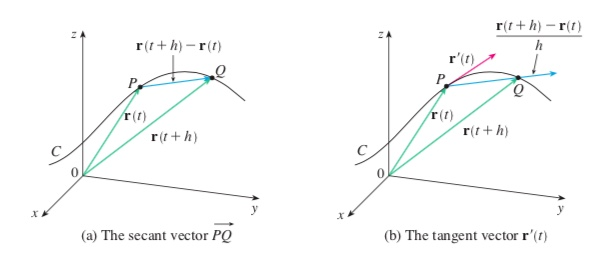
\includegraphics[scale=0.4]{figures_mvc/tangent_vector_secant_vector}
\end{center}
\caption{The derivative $\bbr'(t)$ is the tangent vector to the curve $\bbr$ at $\bbr(t)$.}
\end{figure}
The next theorem shows that we can compute the derivative of a vector-valued function in terms of the derivatives of its component functions.

\begin{thm}[Derivative of a vector-valued function]
	The derivative of a vector-valued function $\bbr(t)=(r_1(t),r_2(t),r_3(t))$ is given by 
	\begin{align*}
		\bbr'(t)=(r_1'(t),r_2'(t),r_3'(t)).
	\end{align*}
\end{thm}

\begin{pf}
By Theorem \ref{thm:limit_of_a_vector-valued_function}
\begin{align*}
	\bbr'(t)&=\lim_{h \to 0}\frac{\bbr(t+h)-\bbr(t)}{h} \\
	&=\lim_{h \to 0}\frac{(r_1(t+h),r_2(t+h),r_3(t+h))-(r_1(t),r_2(t),r_3(t))}{h} \\
	&=\lim_{h \to 0}\frac{(r_1(t+h)-r_1(t),r_2(t+h)-r_2(t),r_3(t+h)-r_3(t))}{h} \\
	&=\lim_{h \to 0}\left(\frac{r_1(t+h)-r_1(t)}{h},\frac{r_2(t+h)-r_2(t)}{h},\frac{r_3(t+h)-r_3(t)}{h}\right) \\
	&=\left(\lim_{h \to 0}\frac{r_1(t+h)-r_1(t)}{h},\lim_{h \to 0}\frac{r_2(t+h)-r_2(t)}{h},\lim_{h \to 0}\frac{r_3(t+h)-r_3(t)}{h}\right) \\
	&=(r_1'(t),r_2'(t),r_3'(t)).
\end{align*}	
\end{pf}

\fixme{Add examples.}

\begin{thm}[Differentiation formulas]
	Let $\bu,\bv$ be differentiable vector-valued functions into $\R^n$, $c$ a constant, and $\varphi:\mathbb{R} \to \mathbb{R}$ a real-valued function. Then
\begin{enumerate}[(1)]
		\item $[\bu(t)+\bv(t)]'=\bu'(t)+\bv'(t)$
		\item $[c\bu(t)]'=c\bu'(t)$
		\item $[\varphi(t)\bu(t)]'=\varphi'(t)\bu(t)+\varphi(t)\bu'(t)$
		\item $[\bu(t)\cdot \bv(t)]'=\bu'(t)\cdot \bv(t)+\bu(t) \cdot \bv'(t)$
		\item $[\bu(t)\times \bv(t)]'=\bu'(t)\times \bv(t)+\bu(t) \times \bv'(t)$ (for $n=3$)
		\item $[\bu(\varphi(t))]'=\varphi'(t)\bu'(\varphi(t))$
	\end{enumerate}	
\end{thm}

\begin{pf}
\fixme{Add proof.}	
\end{pf}


\begin{defn}[Higher derivatives]
	\begin{enumerate}[(a)]
		\item The \emph{second derivative}, $\bbr''$, of a vector-valued function $\bbr$ is the derivative of $\bbr'$: $\bbr''=(\bbr')'$. Thus,
\begin{align*}
	\bbr''(t)=(f''(t), g''(t), h''(t))
\end{align*}
Similarly, for $k$ a positive integer, the $k$th derivative of $\bbr$ is given by the formula
\begin{align*}
	\bbr^{(k)}(t)=(f^{(k)}(t), g^{(k)}(t), h^{(k)}(t)).
\end{align*}
\item A vector-valued function is said to be of class $\mathscr{C}^k$ if its first $k$ derivatives exist and are continuous and of class $\mathscr{C}^\infty$ if all of its derivatives exist. Functions in the class $\mathscr{C}^\infty$ are also called \emph{smooth}.
	\end{enumerate}
\end{defn}

\subsection{Parametrized Curves}
We will now focus on a special class of vector-valued functions, which model the motion of a particle through space. Our interest will primarily be in the geometry of the trajectory of the particle.

\begin{defn}[Parametrized curve]
	Let $I$ be an interval. A \emph{parametrized curve} is a smooth mapping $\bbr:I \to \mathbb{R}^n$. For $n=2$, a curve is also called a \emph{plane curve} while for $n=3$ it is also called a \emph{space curve}. The variable $t$ is called the \emph{parameter}. The image $\bbr(I)$ is called the \emph{trace} of the curve $\bbr$.
\end{defn}

\begin{remark}
If $I$ is an interval containing boundary points, such as $[a,b]$, then we define $f'(a)$ as the right-hand limit
\begin{align*}
	f'(a)=\lim_{h \to 0^+}\frac{f(a+h)-f(a)}{h}
\end{align*}
and, $f'(b)$ as the left-hand limit
\begin{align*}
	f'(b)=\lim_{h \to 0^-}\frac{f(b+h)-f(b)}{h}.
\end{align*}
\end{remark}


\begin{example}
The graph of any smooth function $y=f(x)$ can be written as a parametrized curve by defining
\begin{align*}
	\bbr:\R &\to \R^2 \\
	\bbr(t)&=(t,f(t)).
\end{align*}
For example, the function $y=x^2$ can be written the parametrized curve $\bbr(t)=(t,t^2)$ for all $-\infty < t < \infty$.	The trace of a plane curve can be plotted in \emph{Mathematica} as shown below:

\begin{figure}[h]
	\begin{center}
		\includegraphics[scale=0.5]{figures_mvc/parab_param_plot}
	\end{center}
	\caption{The trace of the plane curve $\bbr(t)=(t,t^2)$.}
\end{figure} 

The particle moves down the parabola from the upper left starting at $t=-\infty$, reaches the origin at $t=0$, and then continues up the parabola to the upper right for all $t>0$.
\end{example}

\begin{exercise}
Sketch the trace of the plane curve $\bbr(t)=(t^2-2t,t+1)$, $-\infty < t < \infty$ in by making a table of the coordinates $(x(t),y(t))$ for integer values of $t$ from $-2 \leq t \leq 4$. Compare your sketch with the curve produced in \emph{Mathematica} using the ``ParametricPlot" command.	
\end{exercise}
{\color{red}
\begin{solution}
	The curve is a parabola, which we can confirm by eliminating $t$ as follows. First, solve for $t$ in terms of $y$ to obtain
\begin{align*}
	y=t+1 \implies y-1=t.
\end{align*}
Substituting into $x(t)$ then gives $x$ in terms of $y$:
\begin{align*}
	x=t^2-2t=(y-1)^2-2(y-1)=y^2-4y+3=(y-2)^2-1.
\end{align*}
which is the equation of a parabola in vertex form, with vertex at $(x,y)=(-1,2)$. 

\begin{figure}[h]
	\begin{center}
		\includegraphics[scale=0.5]{figures_mvc/sideways_parab_mma}
	\end{center}
	\caption{The trace of the plane curve $\bbr(t)=(t^2-2t,t+1)$ from $-2 \leq t \leq 4$.}
\end{figure}

The particle travels upwards along the parabola from $t=-\infty$, reaches the vertex at $t=1$, and then continues upward to the right for $t>0$.
\end{solution}}



\begin{example}\label{ex:unit_circ}
Consider the following three plane curves \fixme{Add definition of derivative for at boundary points of a closed interval.}
\begin{enumerate}[(1)]
	\item $\bbr_1(t)=(\cos t, \sin t), 0 \leq t \leq 2\pi$, 
	\item $\bbr_2(t)=(-\sin 2t, \cos 2t), 0 \leq t \leq 2\pi$,
	\item $\bbr_3(t)=(\cos(-t), \sin(-t)), 0 \leq t \leq 2\pi$.
\end{enumerate}	
For all three curves, $x(t)^2+y(t)^2=1$, so the trace of each curve is the unit circle. However, the curves are different. The reader can easily verify the following by making a table for each curve and sketching the trace:
\begin{enumerate}[(1)]
	\item In $\bbr_1$, the particle begins at $(x,y)=(1,0)$ at $t=0$ and completes one full circle, moving in the counterclockwise direction.
	\item In $\bbr_2$, the particle begins at $(x,y)=(0,1)$ at $t=0$ and completes \emph{two} full circles, moving in the counterclockwise direction.
	\item In $\bbr_3$, the particle begins at $(x,y)=(1,0)$ at $t=0$ and completes one full circle, moving in the \emph{clockwise} direction.
\end{enumerate}
\begin{figure}[h]
	\begin{center}
		\includegraphics[scale=0.4]{figures_mvc/circ_param_plot_mma}
	\end{center}
	\caption{The trace of the curves $\bbr_1,\bbr_2,\bbr_3$.}
\end{figure}
\end{example}
The previous example shows that a parametrized curve is more than just the trace: it is the trace together with a choice of how to traverse the trace of curve.

\begin{example}
Consider now the trace of the plane curve $\bbr(t)=(t^3,t^2)$, $-\infty<t<\infty$.

\begin{figure}[h]
	\begin{center}
		\includegraphics[scale=0.4]{figures_mvc/cusp_mma}
	\end{center}
\end{figure}
Since the component functions are smooth, the reader may be surprised by the cusp at the origin. Solving for $y$ in terms of $x$ by eliminating $t$, we find that $y=x^{2/3}$, which is indeed not differentiable at the origin. Note that $\bbr'(t)=(3t^2,2t)\neq (0,0)$ everywhere except the origin, where the tangent vector vanishes.
\end{example}
 
\begin{defn}[Regular curve]
	Let $\bbr:I \to \R^n$ be a parametrized curve.
	\begin{enumerate}[(a)]
		\item A point where $\bbr'(t)={\bf 0}$ is called a \emph{singular point}, while a point where $\bbr'(t) \neq {\bf 0}$ is called a \emph{regular point}.
		\item A \emph{regular curve} is a curve with no singular points; that is, it is a curve for whice $\bbr'(t) \neq {\bf 0}$ for all $t \in I$.
	\end{enumerate}
\end{defn}
In our study of the differential geometry of curves, we will need the curve to have a tangent vector at every point. Thus, from now on we will assume all curves are regular.

\subsection{Reparametrizations}
Recall the three regular curves from Example \ref{ex:unit_circ}:
\begin{enumerate}[(1)]
	\item $\bbr_1(t)=(\cos t, \sin t), 0 \leq t \leq 2\pi$, 
	\item $\bbr_2(t)=(-\sin 2t, \cos 2t), 0 \leq t \leq 2\pi$,
	\item $\bbr_3(t)=(\cos(-t), \sin(-t)), 0 \leq t \leq 2\pi$.
\end{enumerate}	
We have noticed that all three curves have exactly the same trace; namely, the unit circle. If we are only interested in the geometry of the trace of the curve, then we should view all parametrized curves with the same trace as equivalent. We now formalize this idea.

First, notice that if we define the function
\begin{align*}
	\varphi:[0,2\pi] \to [0,2\pi]
\end{align*}
by 
\begin{align*}
	\varphi(t)=2t+\frac{\pi}{2}
\end{align*}
then we see that $\bbr_2$ is equal to the composition $\bbr_2=\bbr_1 \circ \varphi$, since for all $t \in [0,2\pi]$
\begin{align*}
	\bbr_1(\varphi(t))&=(\cos(2t+\frac{\pi}{2}),\sin(2t+\frac{\pi}{2})) \\
	&=(\cos(2t)\underbrace{\cos(\frac{\pi}{2})}_{=0}-\sin(2t)\underbrace{\sin(\frac{\pi}{2})}_{=1}, \sin(2t)\underbrace{\cos(\frac{\pi}{2})}_{=0}+\cos(2t)\underbrace{\sin(\frac{\pi}{2})}_{=1}) \\
	&=(-\sin(2t),\cos(2t)) \\
	&=\bbr_2(t).
\end{align*}

To understand this relationship, recall that a parametrized curve $\bbr(t)$ is a function which gives the position of the particle at time $t$, with respect to a given clock. If $\varphi$ denotes the time with respect to a different clock, then $\bbr(\varphi)$ gives the position of the particle at time $\varphi$. The particles follow the same trajectory, but are at different positions at different times if the two clocks are not synchronized. In this example, the clocks are related by $\varphi=2t+\frac{\pi}{2}$; that is, the $\varphi$-clock is $\frac{\pi}{2}$ seconds ahead of the $t$-clock (since $\varphi=\frac{\pi}{2}$ when $t=0$), and runs half as fast (since if the time interval between two successive ticks of the $t$-clock is $\Delta t=1$ s, then the time interval between two successive ticks of the $\varphi$-clock is  $\Delta \varphi=2\Delta t=2$ s; that is, if the $t$-clock ticks once every second, then the $\varphi$-clock ticks once every two seconds). Thus, if $\bbr_1(t)$ describes a single trip around the unit circle in the counterclockwise sense at unit speed, then, with respect to the $t$-clock, $\bbr_1(\varphi)=\bbr_2(t)$ describes a particle that is already at $(0,1)$ when $t=0$ and completes two trips around the circle at double speed in $2\pi$ seconds.

\begin{exercise}\label{ex:orient_reve}
Verify that by defining $\varphi:[0,2\pi] \to [0,2\pi]$ by $\varphi(t)=2\pi-t$, then $\bbr_3=\bbr_1 \circ \varphi$. Interpret this as above.	
\end{exercise}

{\color{red}
\begin{solution}
We see that $\bbr_1(\varphi(t))=(\cos(2\pi-t),\sin(2\pi-t))=(\cos(-t),\sin(-t))=\bbr_3(t)$ for all $t$. The $\varphi$-clock is related to the $t$-clock by ``time-reversal"; that is, the clocks run at the same speed, but the $\varphi$ clock runs backwards with respect to the $t$-clock, since $\varphi(t)$ is a decreasing function of $t$ with $\varphi(0)=2\pi$ and $\varphi(2\pi)=0$.	
\end{solution}
}
\begin{defn}[Reparametrization]
	Let $\bbr:I \to \mathbb{R}^n$ be a regular curve. A \emph{reparametrization} of $\bbr$ is a function of the form $\widetilde{\bbr}=\bbr \circ \varphi:\tilde{I} \to \mathbb{R}^n$, where $\tilde{I}$ is an interval and $\varphi:\tilde{I} \to I$ is a smooth bijection with nowhere vanishing derivative ($\varphi'(t) \neq 0$ for all $t \in \tilde{I}$). \footnote{While in each of the examples above we had $\varphi:\tilde{I} \to I$ with $\tilde{I}=I$, these intervals need not be the same. For instance, in Example \ref{ex:orient_reve}, we could have instead taken $\varphi:[0,2\pi] \to [-2\pi,0]$ where $\varphi(t)=-t$.}
\end{defn}

\begin{figure}[h]
	\begin{center}
		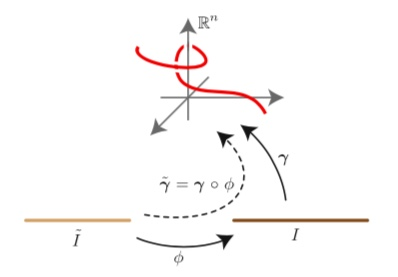
\includegraphics[scale=0.5]{figures_mvc/reparametrization}
	\end{center}
\end{figure}

\begin{remark}
Note that the hypotheses on $\varphi$ are all required to ensure that $\widetilde{\bbr}=\bbr \circ \varphi$ has the same trace as $\bbr$:
\begin{itemize}
	\item The requirement that $\varphi$ is smooth ensures that $\widetilde{\bbr}$ is smooth, since the composition of smooth functions is smooth.
	\item The requirement that $\varphi$ is a bijection is also essential. If $\varphi$ is not surjective, then the trace of $\widetilde{\bbr}$ will only be a proper subset of the trace of $\bbr$. If $\varphi$ is not injective, then $\widetilde{\bbr}$ will have self-intersections at points where $\bbr$ does not (since if $\varphi(t_1)=\varphi(t_2)$ for $t_1 \neq t_2$, then even if $\bbr(t_1) \neq \bbr(t_2)$, we will have $\widetilde{\bbr}(\varphi(t_1))=\widetilde{\bbr}(\varphi(t_2))$). \fixme{Maybe say this better or give an example.}
	\item The requirement that $\varphi'(t) \neq 0$ for all $t$ ensures that $\widetilde{\bbr}(t)$ is regular, since if $\bbr(t)$ is regular and $\varphi'(t) \neq 0$, then by the chain rule
	\begin{align*}
		\widetilde{\bbr}'(t)=\varphi'(t)\bbr'(t) \neq 0.
	\end{align*}
\end{itemize}
\fixme{Give examples or an exercise in which each of these separately fail.}
\end{remark}

\begin{prop}[Reparametrized curves are equivalent]
The relation $\widetilde{\bbr} \sim \bbr$ if $\widetilde{\bbr}$ is a reparametrization of $\bbr$ is an equivalence relation. 	
\end{prop}

\begin{pf}
	\begin{enumerate}[(1)]
		\item (Reflexivity) Let $\bbr:I \to \R^n$ be a parametrized curve. Take $\varphi=id_I:T \to I$ to be the identity map on $I$. This is a smooth bijection, and since $id_I(t)=t$, $id_I'(t)=1 \neq 0$ for all $t \in I$. Since $\bbr=\bbr \circ id_I$, $\bbr \sim \bbr$. Thus, $\sim$ is reflexive.
		\item (Symmetry) Suppose $\bbr:I \to \R^n$ and $\widetilde{\bbr}:\tilde{I} \to \R^n$ are parametrized curves with $\widetilde{\bbr} \sim \bbr$. Then there exists a smooth bijection $\varphi: \tilde{I} \to I$ with $\varphi'(t) \neq 0$ for all $t \in \tilde{I}$. It follows from the Inverse Function Theorem that $\varphi$ has a smooth inverse, $\varphi^{-1} :I \to \tilde{I}$, where $(\varphi^{-1})'(t)=1/\varphi'(t)$ Since $\varphi'(t)$ is never zero, neither is $(\varphi^{-1})'(t)$. \footnote{The \emph{Inverse Function Theorem} states that if $f:\R \to \R$ is continuously differentiable with $f'(a) \neq 0$ then $f$ is invertible in a neighborhood of $a$, the inverse is continuously differentiable, and the derivative of the inverse function at $b=f(a)$ is the reciprocal of the derivative of $f$ at $a$. Applying this to the $k$-th derivative, it follows as a corollary that we can replace ``continuously differentiable" everywhere in the theorem above by ``smooth". The \emph{Gluing Lemma} then allows us to patch together the inverse on each neighborhood into an inverse defined on the entire interval $I$.} This proves that $\widetilde{\bbr} \sim \bbr$ implies that $\bbr \sim \widetilde{\bbr}$. Thus, $\sim$ is symmetric.
		\item (Transitivity) Let
		\begin{align*}
			\bbr_1:I_1 &\to \R^n, \\
			\bbr_2:I_2 &\to \R^n, \\
			\bbr_3:I_3 &\to \R^n, \\
		\end{align*}
		be parametrized curves and suppose $\bbr_1 \sim \bbr_2$ and $\bbr_2 \sim \bbr_3$. Then there exist smooth bijections 
		\begin{align*}
			\varphi:I_2 &\to I_1, \\
			\psi:I_3 &\to I_2
		\end{align*} 
		with nowhere vanishing first derivatives such that
		\begin{align*}
			\bbr_2&=\bbr_1 \circ \varphi, \\
			\bbr_3&=\bbr_2 \circ \psi
		\end{align*}
		Then $\varphi \circ \psi:I_3 \to I_1$ is a smooth bijection with nowhere vanishing derivative such that
		\begin{align*}
			\bbr_3=\bbr_1 \circ \varphi \circ \psi.
		\end{align*}
		Thus, $\bbr_1 \sim \bbr_3$.
	\end{enumerate}
	This shows that $\sim$ is reflexive, symmetric, and transitive, and is therefore an equivalence relation.
\end{pf}
\begin{defn}[Curve]
	The we call the equivalence class
	\begin{align*}
		[\bbr]\equiv \{\widetilde{\bbr}:\widetilde{\bbr}=\bbr \circ \varphi \text{ for some } \varphi\}
	\end{align*} 
 a \emph{curve} in $\R^n$. Any parametrized curve $\widetilde{\bbr}(t)$ in $[\bbr]$ is said to be a \emph{representative} of the equivalence class $[\bbr]$. \fixme{Show that if two curves have the same trace, then they are equivalent.}
\end{defn}
Let $\bbr(t)$ be a parametrized curve and let $\widetilde{\bbr}=\bbr \circ \varphi$ be a reparametrization of $\bbr(t)$. Since $\varphi'(t)$ is nowhere 0, $\varphi$ must be either monotonically increasing ($\varphi'>0$) or monotonically decreasing ($\varphi'<0$) on all of $\tilde{I}$.

\begin{defn}[Oriented curves]
A reparametrization $\widetilde{\bbr}=\bbr \circ \varphi$ is said to be \emph{orientation-preserving} if $\varphi'>0$ and \emph{orientation-reversing} if $\varphi'<0$. Thus, each curve $[\bbr]$ is partitioned into two subsets
\begin{align*}
	[\bbr]_+&=\{\widetilde{\bbr}:\widetilde{\bbr}=\bbr \circ \varphi \text{ with } \varphi'>0\}, \\
	[\bbr]_-&=\{\widetilde{\bbr}:\widetilde{\bbr}=\bbr \circ \varphi \text{ with } \varphi'<0\}. \\
\end{align*}
Each subset is called an \emph{oriented curve}. A choice of orientation of a curve $[\bbr]$ is a choice of one of these two subsets.
\end{defn}

\begin{example}
Consider again three parametrized curves from Example \ref{ex:unit_circ} and :
\begin{enumerate}[(1)]
	\item $\bbr_1(t)=(\cos t, \sin t), 0 \leq t \leq 2\pi$, 
	\item $\bbr_2(t)=(-\sin 2t, \cos 2t), 0 \leq t \leq 2\pi$,
	\item $\bbr_3(t)=(\cos(-t), \sin(-t)), 0 \leq t \leq 2\pi$.
\end{enumerate}	
We have seen that $\bbr_2=\bbr_1 \circ \varphi$ where $\varphi(t)=2t+\frac{\pi}{2}$. Since $\varphi'(t)=2>0$, these two curves have the same orientation (i.e., they are representatives of the same oriented curve). We also saw that $\bbr_3=\bbr_1 \circ \psi$ where $\psi(t)=2\pi-t$. Since $\psi'(t)=-1<0$, these two curves have opposite orientations.
\end{example}
\fixme{Add exercises.}

\subsection{Arc Length}
We have just seen that a given curve can be parametrized in many ways. Out of these many options, there is a natural choice for the parameter $t$, namely, the \emph{arc length} measured from any point $\bbr_0$ on the curve. This is because the arc length is an \emph{invariant} of the curve, which is independent of the parametrization. For a curve given by the graph of a function $y=f(x)$, the arc length from $a$ to $b$ is given by
\begin{align}\label{eq:arc_leng_f_x}
	s=\int_a^b\sqrt{1+(f'(x))^2}dx.
\end{align}
Writing the function as a parametrized curve $\bbr(t)=(t,f(t))$, we have $\bbr'(t)=(1,f'(t))$ and $||\bbr'(t)||=\sqrt{1+(f'(t))^2}$, so we can write Equation \eqref{eq:arc_leng_f_x} as
\begin{align}\label{eq:arc_length_gen}
	s=\int_a^b||\bbr'(t)||dt.
\end{align}
\fixme{Add example.}
How do we compute the arc length if $\bbr(t)$ is not the graph of a function? If $\bbr(t)$ is not the graph of a function, it turns out that Equation \eqref{eq:arc_length_gen} is still valid. In this case, we obtain the formula as the limit of a sequence of polygonal approximations of the curve (the proof is given in Appendix \ref{app:arc_length}). 

\begin{defn}{Arc length}\label{def:arc_length}
Let $\bbr:[a,b] \to \R^n$ be a regular curve. We define the \emph{arc length} between the points $\bbr(a)$ and $\bbr(b)$ on the curve by
\begin{align*}
	s=\int_a^b||\bbr'(t)||dt.
\end{align*}	
\end{defn}

\begin{example}\label{ex:unit_circl_ex}
We now compute the arc length along the portion of the unit circle from $(1,0)$ to $(0,1)$. If we use the parametrization
\begin{align*}
	\bbr_1(t)=(\cos t,\sin t), 0 \leq t \leq \frac{\pi}{2},
\end{align*}	
then we have
\begin{align*}
	\bbr_1'(t)&=(-\sin t,\cos t), \\
	||\bbr_1'(t)||&=\sqrt{(-\sin t)^2+(\cos t)^2}=\sqrt{1}=1.
\end{align*}
Equation \eqref{eq:arc_length_gen} then gives
\begin{align*}
	s=\int_0^{\frac{\pi}{2}}||\bbr_1'(t)||dt=\int_0^{\frac{\pi}{2}}dt=\frac{\pi}{2}.
\end{align*}
\end{example}

\begin{exercise}
Use the parametrization $\bbr_2(t)=(\cos(2t),\sin(2t)), 0 \leq t \leq \frac{\pi}{4}$ to compute the arc length of the same portion of the unit circle as in Example \ref{ex:unit_circl_ex}. Verify that you get the same answer.	
\end{exercise}

{\color{red}
\begin{solution}
	Using the parametrization $\bbr_2(t)=(\cos(2t),\sin(2t))$, $0 \leq t \leq \frac{\pi}{4}$, we have
	\begin{align*}
		\bbr_2'(t)&=(-2\sin(2t),2\cos(2t)), \\
		||\bbr_2'(t)||&=\sqrt{4\sin^2(2t)+4\cos^2(2t)}=\sqrt{4(\sin^2(2t)+\cos^2(2t))}=\sqrt{4}=2
	\end{align*} 
	and therefore
	\begin{align*}
		s=\int_0^{\frac{\pi}{4}}||\bbr_2'(t)||dt=2\int_0^{\frac{\pi}{4}}dt=2\cdot \frac{\pi}{4}=\frac{\pi}{2}.
	\end{align*}
\end{solution}}

\begin{exercise}
A \emph{logarithmic spiral} is a plane curve of the form $\bbr(t)=c(e^{\lambda t}\cos t,e^{\lambda t}\sin t)$, $t \in \mathbb{R}$ where $c,\lambda \in \mathbb{R}$ and $c \neq 0$. Below is the restriction of $\bbr(t)$ to $[0,\infty)$ with $\lambda <0$.	

\begin{figure}[h]
	\begin{center}
		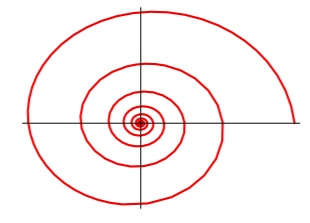
\includegraphics[scale=0.5]{figures_mvc/log_spiral}
	\end{center}
\end{figure}
Use an improper integral to prove that such a restriction has finite arc length even though it makes infinitely many loops around the origin.
\end{exercise}

{\color{red}
\begin{solution}
	We have
	\begin{align*}
		\bbr'(t)&=c(\lambda e^{\lambda t}\cos t-e^{\lambda t}\sin t,\lambda e^{\lambda t}\sin t+e^{\lambda t}\cos t) \\
		&=ce^{\lambda t}(\lambda \cos t-\sin t, \lambda \sin t+\cos t)
	\end{align*}
	and therefore
	\begin{align*}
		||\bbr'(t)||&=|c|e^{\lambda t}\sqrt{(\lambda \cos t-\sin t)^2+(\lambda \sin t+\cos t)^2} \\
		&=|c|e^{\lambda t}\sqrt{\lambda^2\cos^2 t+\sin^2 t-2\lambda \sin t \cos t+\lambda^2\sin^2 t+ \cos ^2 t+2\lambda \sin t\cos t} \\
		&=|c|e^{\lambda t}\sqrt{\lambda^2+1}.
	\end{align*}
	The arc length is then given by the integral
	\begin{align*}
		s=\int_0^\infty ||\bbr'(t)||dt=|c|\sqrt{\lambda^2+1}\int_0^\infty e^{-|\lambda|t}dt.
	\end{align*}
	Substituting
	\begin{align*}
		u=-|\lambda|t, \ du=-|\lambda|dt,
	\end{align*}
	this becomes
	\begin{align*}
		s&=-\frac{|c|\sqrt{\lambda^2+1}}{|\lambda|}\int_0^{-\infty}e^{u}du \\
		&=-\frac{|c|\sqrt{\lambda^2+1}}{|\lambda|}\lim_{k \to -\infty}(e^k-1) \\
		&=-\frac{|c|\sqrt{\lambda^2+1}}{|\lambda|}(0-1) \\
		&=\frac{|c|\sqrt{\lambda^2+1}}{|\lambda|}.
	\end{align*}
\end{solution}}

\begin{prop}[Invariance of arc length]
	The arc length is independent of parametrization.
\end{prop}

\begin{pf}
Let $\widetilde{\bbr}=\bbr \circ \varphi$ be a reparametrization of $\bbr$. Then since
\begin{align*}
	\widetilde{\bbr}'(t)&=[\bbr(\varphi(t))]'=\varphi'(t)\bbr'(\varphi(t)),
\end{align*}
we have
\begin{align*}
	s&=\int_{t_0}^{t_1}||\widetilde{\bbr}'(t)||dt \\
	&=\int_{t_0}^{t_1}||\varphi'(t)\bbr'(\varphi(t))||dt \\
	&=\int_{t_0}^{t_1}||\bbr'(\varphi(t))|| \ |\varphi'(t)|dt \\
\end{align*}	
If $\varphi'(t)>0$, then $|\varphi'(t)|=\varphi'(t)$ and by substituting
\begin{align*}
	u=\varphi(t), \ du=\varphi'(t)dt
\end{align*}
we obtain
\begin{align*}
	s=\int_{\varphi(t_0)}^{\varphi(t_1)}||\bbr'(u)||du.
\end{align*}
If $\varphi'(t)<0$, then $|\varphi'(t)|=-\varphi'(t)$ and the same substitution gives
\begin{align*}
	s=-\int_{\varphi(t_0)}^{\varphi(t_1)}||\bbr'(u)||du=\int_{\varphi(t_0)}^{\varphi(t_1)}||\bbr'(u)||du.
\end{align*}
\fixme{Include figure?}
\end{pf}

\begin{prop}[Any regular curve can be parametrized by arc length]
	Any regular curve $\bbr:I \to \R^n$ can be parametrized by arc length.
\end{prop}

\begin{pf}
Choose $t_0 \in I$ and consider the arc length function $s:I \to \R$ defined by
\begin{align*}
	s(t)=\int_{t_0}^t||\bbr'(u)||du. 
\end{align*}	
Let $\tilde{I}=s(I)$ denote the image of $I$ under $s$. By the Fundamental Theorem of Calculus, $s'(t)=||\bbr'(t)|| \neq 0$ (since the curve is regular), so by the Inverse Function Theorem $s$ has an inverse $\varphi:\tilde{I} \to I$, which is also a smooth bijection with a nowhere-vanishing derivative. Then $\widetilde{\bbr}=\bbr \circ \varphi$ is parametrized by arc length, since $\bbr(\varphi(s))$ is the position of a point along the curve at the time when it achieves arc length $s$ measured from $t_0$.
\end{pf}

\begin{example}\label{ex:helix_param_by_arc_length}
Consider the helix $\bbr(t)=(\cos t, \sin t, t)$, $t \in \R$. 
\begin{figure}[h]
	\begin{center}
		\includegraphics[scale=0.5]{figures_mvc/helix_fig}
	\end{center}
\end{figure}

 Let us reparametrize the helix with respect to the arc length measured from $(1,0,0)$ in the direction of increasing $t$. Since $\bbr(0)=(1,0,0)$, following the proof above we define
\begin{align*}
	s(t)=\int_0^t||\bbr'(u)||du.
\end{align*}
Since $\bbr'(u)=(-\sin u,\cos u,1)$, we have $||\bbr'(u)||=\sqrt{2}$ and therefore
\begin{align*}
	s(t)&=\int_0^t||\bbr'(u)||du \\
	&=\sqrt{2}\int_0^t du \\
	&=\sqrt{2}t.
\end{align*}
The inverse function is then easily obtained:
\begin{align*}
	\varphi(s)=\frac{s}{\sqrt{2}}
\end{align*}
and 
\begin{align*}
	\bbr(\varphi(s))=\left(\cos\left(\frac{s}{\sqrt{2}}\right),\sin\left(\frac{s}{\sqrt{2}}\right),\frac{s}{\sqrt{2}}\right).
\end{align*}
\end{example}

\begin{example}
Let's reparametrzie the plane curve $\bbr(t)=(\cos(3t),\sin(2t))$ with respect to arc length measured from $(1,0)$ in the direction of increasing $t$. Since
	\begin{align*}
		\bbr'(t)&=(-3\sin(3t),2\cos(2t)) \\
		||\bbr'(t)||&=\sqrt{9\sin^2(3t)+4^2\cos(2t)},
	\end{align*}
	the arc length function is given by
	\begin{align*}
		s(t)=\int_0^t\sqrt{9\sin^2(3t)+4\cos^2(2t)}dt
	\end{align*}
	This integral cannot be evaluated in terms of elementary functions. \fixme{Explain what this means.} This example illustrates that, while our proof gave an explicit method to parametrize any curve by arc length, in practice it is usually not computationally reasonable to implement. However, we will use the fact that every curve can be parametrized by arc length for theoretical purposes.
\end{example}

\begin{prop}
	A curve parametrized by arc length is a \emph{unit speed curve}; that is, $||\bbr'(t)||=1$ for all $t \in I$.
\end{prop}

\begin{proof}
	If $\bbr$ is parametrized by arc length, then by the Fundamental Theorem of Calculus
	\begin{align*}
		s'(t)=\frac{d}{dt}\int_{t_0}^t||\bbr'(u)||du=||\bbr'(t)||=1.
	\end{align*}
	Conversely, suppose $||\bbr'(t)||=1$ for all $t$. Then
	\begin{align*}
		s(t)=\int_{t_0}^t||\bbr'(u)||du=\int_{t_0}^tdu=t-t_0
	\end{align*}
	so $t$ is equal to the arc length accumulated from the point $t_0$.
\end{proof}

\begin{exercise}
Verify that the helix parametrized by arc length in Example \ref{ex:helix_param_by_arc_length} is a unit speed curve.	
\end{exercise}

{\color{red}
\begin{solution}
We have $\bbr'(s)=\frac{1}{\sqrt{2}}(-\sin(\frac{s}{\sqrt{2}}), \cos(\frac{s}{\sqrt{2}}),1)$ and therefore 
\begin{align*}
	||\bbr'(s)||&=\frac{1}{\sqrt{2}}\sqrt{\sin^2(\frac{s}{\sqrt{2}})+\cos^2(\frac{s}{\sqrt{2}})+1} \\
	&=\frac{1}{\sqrt{2}}\sqrt{2} \\
	&=1.
\end{align*}	
\end{solution}

}
\subsection{Curvature}
In this section, we will quantify how sharply a curve ``bends" at each point. This will lead us to define a function called the \emph{curvature function} for the curve.

\subsection{Curvature of a unit speed curve}
We begin by considering curves parametrized by arc length. To define the curvature function, we will need the following lemma.
\begin{lem}\label{lem:some_dot_products}
Let $\bu, \bv:I \to \R^n$ be a pair of curves.
\begin{enumerate}[(a)]
	\item If $\bu$ has constant nonzero length (that is, if $||\bu(t)||=c>0$ for all $t \in I$), then $\bu'(t)$ is orthogonal to $\bu(t)$ for all $t \in I$.
	\item If $\bu(t)$ is orthogonal to $\bv(t)$ for all $t \in I$, then
	\begin{align*}
		\bu'(t) \cdot \bv(t)=-\bu(t) \cdot \bv'(t)=0
	\end{align*}
	for all $t \in I$.
\end{enumerate}	
\end{lem}

\begin{proof}
	\begin{enumerate}[(1)]
		\item Suppose $||\bu(t)||=c$ for all $t$. Differentiating both sides, gives $||\bu(t)||'=0$. That is,
		\begin{align*}
			0&=||\bu(t)||' \\
			&=\sqrt{\bu(t) \cdot \bu(t)}' \\
			&=\frac{2\bu'(t) \cdot \bu(t)}{2\sqrt{\bu(t) \cdot \bu(t)}} \\
			&=\frac{\bu'(t) \cdot \bu(t)}{||\bu(t)||} \\
			&=\frac{\bu'(t) \cdot \bu(t)}{c} \\
		\end{align*}
		and therefore $\bu'(t) \cdot \bu(t)=0$ for all $t$.
		\item Suppose $\bu(t) \cdot \bv(t)=0$ for all $t$. Differentiating both sides, we obtain
		\begin{align*}
			0&=\bu'(t) \cdot \bv(t)+\bu(t)+\bv'(t)
		\end{align*}
		and therefore
		\begin{align*}
			\bu'(t) \cdot \bv(t)=-\bu(t)+\bv'(t)
		\end{align*}
		for all $t$.
	\end{enumerate}
\end{proof}

Note that both of these hypotheses of Lemma \ref{lem:some_dot_products} are true for an orthonormal set of vectors $\{\bu,\bv\}$.

Let $\bbr:I \to \R^n$ be a curve parametrized by arc length. Since $\bbr'(s)$ has unit length, by part (a) of Lemma \ref{lem:some_dot_products}, $\bbr''(s)$ is orthogonal to $\bbr'(s)$. Thus, $||\bbr''(s)||$ measures the rate at which the curve is pulling away from the tangent line at $\bbr(s)$.

\begin{defn}[Curvature]\label{def:curvature}
	Let $\bbr:I \to \R^n$ be a curve parametrized by arc length $s \in I$. Define the \emph{curvature function} $\kappa:I \to [0,\infty)$ by $\kappa(s)=||\bbr''(s)||$. The number $\kappa(s)$ is called the \emph{curvature} of the curve $\bbr$ at $s$.
	\end{defn}

\begin{example}\label{ex:line_circle}
\begin{enumerate}[(a)]
	\item If $\bbr$ is a straight line, then $\bbr(s)=\bbr'(s_0)s+\bbr(s_0)$, where $\bbr(s_0), \bbr'(s_0)$ are constant vectors and we have $\kappa(s)=\bbr''(s)\equiv 0$. Conversely, if $\kappa=||\bbr''(s)||\equiv 0$, then integrating twice gives $\bbr(s)=\bbr'(s_0)s+\bbr(s_0)$, so the curve is a straight line.

\item If $\bbr(s)=(R\cos(\frac{s}{R}),R\sin(\frac{s}{R}))$ is a circle of radius $R$, then
\begin{align*}
	\bbr''(s)=(-\frac{1}{R}\cos(\frac{s}{R}),-\frac{1}{R}\sin(\frac{s}{R}))
\end{align*}
and therefore
\begin{align*}
	\kappa(s)=||\bbr''(s)||=\frac{1}{R}.
\end{align*}
\end{enumerate}	
\end{example}

\begin{defn}[Unit normal vector]
At points where $\kappa(s) \neq 0$, the vector
\begin{align*}
	\mathbf{\hat{n}}(s)=\frac{\bbr''(s)}{||\bbr''(s)||}
\end{align*}
is a unit vector orthogonal to $\bbr'(s)$. This is called the \emph{unit normal vector} to $\bbr$ at $s$.	
\end{defn}

\subsection{Osculating Plane}
Let $\bbr(s)$ be a unit-speed curve. Consider a point $s_0$ where $\kappa(s_0) \neq 0$. Then, for sufficiently small $h=s-s_0$, we can approximate $\bbr(s)$ by its second-order Taylor polynomial:
\begin{align*}
	\bbr(s_0+h)&=\bbr(s_0)+h\bbr'(s_0)+\frac{h^2}{2}\bbr''(s_0)+\mathbf{E}(h),  \\
	\bbr(s_0+h)&=\bbr(s_0)+h\mathbf{\hat{t}}+\frac{h^2}{2}\kappa(s_0)\un(s_0)+\mathbf{E}(h),  \\
\end{align*}
where $\lim_{h \to 0}\frac{||\mathbf{E}(h)||}{h^2}=0$. Thus, sufficiently near $\bbr(s_0)$, the trace of a curve lies in the plane spanned by $\{\ut(s_0),\un(s_0)\}$, called the \emph{osculating plane at $\bbr(s_0)$}. With respect to the coordinate $\bbr(s_0+h)-\bbr(s_0)$ centered at $\bbr(s_0)$, the trace of the curve in the osculating plane is given by 
\begin{align*}
	\{(h,\frac{\kappa(s_0)}{2}h^2):-\epsilon < h < \epsilon\} \subseteq \R^2,
\end{align*}
which is a parabola $y=\frac{\kappa(s_0)}{2}x^2$ whose vertex is at the origin and whose concavity is $y''=\kappa(s_0)$.

\begin{figure}[h]
	\begin{center}
		\includegraphics[scale=0.5]{figures_mvc/parab_curvature}
	\end{center}
	\caption{The trace of $\bbr$ is approximated near $\bbr(s_0)$ by the parabola with concavity $\kappa(s_0)$ in the osculating plane.}
\end{figure}

The trace of the curve is also well approximated by a certain circle in the osculated plane. 

\begin{defn}[Osculating circle]
	The \emph{osculating circle} to is the circle of radius $\kappa(s_0)$ in the osculating plane centered at $\bbr(s_0)+\frac{1}{\kappa(s_0)}\un$.
\end{defn}

\begin{figure}[h]
	\begin{center}
		\includegraphics[scale=0.5]{figures_mvc/osc_circl}
	\end{center}
	\caption{The osculating circle for a plane curve (left) and a space curve (right).}
\end{figure}
Thus, we may also interpret the curvature as the radius of the osculating circle. \fixme{Add Exercise 1.42?}

At points where $\kappa(s)=0$, the normal vector (and therefore the osculating plane) is not defined. To proceed with our analysis, we will need the osculating plane, so from now on we will only consider curves for which $\kappa(s) \neq 0$ for all $s \in I$.

\subsection{Arbitrary parametrizations}
As noted previously, in practice it is often too difficult to parametrize a curve by arc length, and we are forced to work with other parametrizations.

Let $\bbr:I \to \R^n$ be a curve with an arbitrary parametrization $t \in I$. One might guess that the curvature. Since the speed $||\bbr'(t)||$ is no longer constant, the acceleration vector $\bbr''(t)$ will have a nonzero component in the direction of the velocity vector $\bbr'(t)$. We might therefore be tempted to define the curvature function $\kappa(t)$ as the magnitude of the component of the acceleration perpendicular to $\bbr'(t)$; that is, to define $\kappa(t):=||\bbr_\perp''(t)||$, where
\begin{align*}
	\bbr''_\perp(t)&=\bbr''(t)-\text{proj}_{\bbr'(t)}\bbr''(t) \\
	&=\bbr''(t)-\frac{\bbr''(t)\cdot \bbr'(t)}{\bbr'(t)\cdot \bbr'(t)}\bbr'(t). 
\end{align*}
 However, this definition is problematic, as the next example shows.

\begin{example}\label{ex:curvature_arb_bad_def}
Consider the parabola which is the graph of $y=x^2$. Describe the parabola as a parametrized curve in the following two  parametrizations,	
\begin{align*}
	\bbr_1(t)&=(t,t^2), \hspace{2.5cm} t \in \R, \\
	\bbr_2(t)&=(2t-2,(2t-2)^2), \hspace{0.5cm} t \in \R.
\end{align*}
In the first parametrization, the origin is the point $\bbr(0)=(0,0)$. Since
\begin{align*}
	\bbr_1'(t)&=(1,2t), \\
	\bbr_1''(t)&=(0,2),
\end{align*}
\begin{align*}
	\bbr''_{1 \ \perp}(0)&=(0,2)-\frac{(0,2)\cdot (1,0)}{(1,0)\cdot (1,0)}(1,0) \\
	&=(0,2),
\end{align*}
and therefore $\kappa(0)=||\bbr''_{1 \ \perp}(0)||=2$.

In the second parametrization, the origin is $\bbr_2(1)=(0,0)$. Since
\begin{align*}
	\bbr_2'(t)&=(2,4(2t-2))=(2,8t-8) \\
	\bbr_2''(t)&=(0,8) \\
\end{align*}
we have
\begin{align*}
	\bbr_{2 \ \perp}''(1)&=(0,8)-\frac{(0,8)\cdot (2,0)}{(2,0) \cdot (2,0)}(2,0) \\
	&=(0,8)
\end{align*}
and therefore
\begin{align*}
	\kappa(1)=||\bbr_{2 \ \perp}''(1)||=8.
\end{align*}
Using our definition of $\kappa(t)$, we have just obtained \emph{different} values of the curvature at the origin of the parabola by using different parametrizations. The curvature should be a geometric property of the curve that does not depend on parametrization, so this definition turns out to be bad. 
\end{example}

To find a satisfactory definition of curvature, we need to study more carefully the dependence of the derivatives of $\bbr(t)$ on parametrization. Let $\bbr:I \to \R^n$ be a regular curve with an arbitrary paramtrization, and let $\tilde{\bbr}=\bbr \circ \varphi$ be a reparametrization of $\bbr$. Then, by the chain rule,
\begin{align*}
	\widetilde{\bbr}'(t)&=\bbr'(\varphi(t))\varphi'(t), \\
	\widetilde{\bbr}''(t)&=\bbr''(\varphi(t))(\varphi'(t))^2+\bbr'(\varphi(t))\varphi''(t), \\
\widetilde{\bbr}''_\perp(t)&=\bbr''_\perp(\varphi(t))(\varphi'(t))^2.
\end{align*}
From these expressions, we see that the quantity
\begin{align}\label{eq:curvature_arb_param}
	\frac{||\bbr''_\perp(t)||}{||\bbr'(t)||^2}
\end{align}
is invariant under reparametrizations. Moreover, when $t=s$ is the arc length, $||\bbr'(s)||=1$ and $\bbr''(s)=\bbr''_\perp(s)$, so the expression in \eqref{eq:curvature_arb_param} agrees with our definition of the curvature function of a unit speed curve in Definition \ref{def:curvature}.

Thus, we arrive at our definition of the curvature function in an arbitrary parametrization.
\begin{defn}[Curvature in an arbitrary parametrization]
	Let $\bbr:I \to \R^n$ be a regular curve with an arbitrary parametrization $t \in I$. We define the \emph{curvature function} $\kappa:I \to [0,\infty)$ for all $t \in I$ by
	\begin{align}\label{eq:curvature_function_defi}
		\kappa(t)=\frac{||\bbr''_\perp(t)||}{||\bbr'(t)||^2}.
	\end{align}
\end{defn}
Rewriting \eqref{eq:curvature_function_defi} as 
\begin{align*}
	||\bbr_\perp''(t)||=\kappa(t)||\bbr'(t)||^2,
\end{align*}
this expression says, in physical terms, that the magnitude of the centripetal acceleration at $t$ depends not only on the curvature, but also on the speed at $t$. This explains the results of Example \ref{ex:curvature_arb_bad_def}.

\begin{defn}[Unit tangent and Unit normal in an arbitrary parametrization]
	Let $\bbr:I \to \R^n$ be a regular curve with an arbitrary parametrization and let $t \in I$ be a point where $\kappa(t) \neq 0$. We define the \emph{unit tangent} and \emph{unit normal vectors} at $t$ to be 
	\begin{align*}
		\ut(t)=\frac{\bbr'(t)}{||\bbr'(t)||}, \hspace{0.5cm} \un(t)=\frac{\bbr''_\perp(t)}{||\bbr''_\perp(t)||}.
	\end{align*} 
\end{defn}

The next proposition shows that we can compute the unit normal vector in terms of the unit tangent vector.

\begin{prop}
Let $\bbr:I \to \R^n$ be a regular curve. For any point where $\kappa(t) \neq 0$, we have
\begin{align*}
	\un(t)=\frac{\ut'(t)}{||\ut'(t)||}.
\end{align*}
\end{prop}

\begin{proof}
	By the quotient rule,
	\begin{align*}
		\ut'(t)=\frac{||\bbr'(t)||\bbr''(t)-\bbr'(t)||\bbr'(t)||'}{||\bbr'(t)||^2}.
	\end{align*}
	Now
	\begin{align*}
		||\bbr'(t)||'&=\frac{d}{dt}(\bbr'(t) \cdot \bbr'(t))^{1/2} \\
		&=\frac{1}{2}(\bbr'(t) \cdot \bbr'(t))^{-1/2}(2\bbr''(t) \cdot \bbr'(t)) \\
		&=\frac{\bbr''(t) \cdot \bbr'(t)}{||\bbr'(t)||} \\
	\end{align*}
	so we have
	\begin{align*}
		\ut'(t)&=\frac{||\bbr'(t)||\bbr''(t)-\bbr'(t)||\bbr'(t)||'}{||\bbr'(t)||^2} \\
		&=\frac{\bbr''(t)}{||\bbr'(t)||}-\frac{\bbr''(t) \cdot \bbr'(t)}{||\bbr'(t)||^3}\bbr'(t) \\
		&=\frac{1}{||\bbr'(t)||}\left(\bbr''(t)-\frac{\bbr''(t) \cdot \bbr'(t)}{||\bbr'(t)||^2}\bbr'(t)\right) \\
		&=\frac{\bbr''_\perp(t)}{||\bbr'(t)||}.
	\end{align*}
	and therefore
	\begin{align*}
		\frac{\ut'(t)}{||\ut'(t)||}&=\frac{\frac{\bbr''_\perp(t)}{||\bbr'(t)||}}{\frac{||\bbr''_\perp(t)||}{||\bbr'(t)||}} \\
		&=\frac{\bbr''_\perp(t)}{||\bbr''_\perp(t)||} \\
		&\equiv \un(t).
	\end{align*}
\end{proof}

\subsection{Plane curves}
Our results so far about curves in $\R^n$ have been valid for all $n$. In this section, we consider the special case $n=2$. This is the only dimension in which the terms ``clockwise" and ``counterclockwise" make sense for describing how a regular curve is turning.

\begin{prop}
The map $R: \R^2 \to \R^2$ defined by $R(x,y)=(-y,x)$ is an isomorphism.
\end{prop}

\begin{proof}
	The map $R$ is the same as multiplication by the matrix 
	\begin{align*}
		\begin{bmatrix}
			0 & -1 \\
			1 & 0
		\end{bmatrix},
	\end{align*}
	which is linear. The kernel of this map is $\{(0,0)\}$, so $R$ is injective. Given any $(x,y) \in \R^2$, we see that $(x,y)=R(y,-x)$, hence $R$ is also surjective. Thus, $R$ is an isomorphism. 
\end{proof}
Geometrically, $R$ rotates each vector $(x,y) \in \R^2$ counterclockwise by $90^\circ$. One can immediately check that $R^2(\bv)\equiv R(R(\bv))=-\bv$ for all $\bv \in \R^2$.

Suppose now that $\bbr:I \to \R^2$ is a unit-speed curve. Then, for all $s \in I$, by Lemma \ref{lem:some_dot_products} $\bbr''(t)$ and $R(\bbr'(t))$ are both orthogonal to $\bbr'(t)$, so they must be parallel. We can therefore write
\begin{align}\label{eq:acc_signed_curvature}
	\bbr''(t)=\kappa_s(t) R(\bbr'(t))
\end{align}
for some scalar $\kappa_s(t) \in \R$. We call $\kappa_s:I \to \R$ the \emph{signed curvature function}. It is negative if the curve is turning clockwise at $t$, and positive if it is turning counterclockwise, as shown below:
\begin{figure}[h]
	\begin{center}
		\includegraphics[scale=0.5]{figures_mvc/signed_curvature_fcn}
	\end{center}
	\caption{Signed curvature is positive when the path is turning counterclockwise, and negative when turning clockwise.}
\end{figure}
This measurement is called ``signed curvature" because its sign is interpreted as above, while its absolute value equals the curvature:

\begin{prop}
Let $\bbr:I \to \R^2$ be a regular unit-speed plane curve. Then $|\kappa_s(t)|=\kappa(t)$.	
\end{prop}

\begin{proof}
	Since $||R(\bbr'(t))||=||\bbr'(t)||=1$,
	\begin{align*}
		\kappa(t)=||\bbr''(t)||=||\kappa_s(t)R(\bbr'(t))||=|\kappa_s(t)| \ ||R(\bbr'(t))||=|\kappa_s(t)|.
	\end{align*}
\end{proof}

Taking the dot product of \eqref{eq:acc_signed_curvature} with $R(\bbr'(t))$, we obtain
\begin{align*}
	\bbr''(t) \cdot R(\bbr'(t))&=\kappa_s(t) R(\bbr'(t)) \cdot R(\bbr'(t))\\
	&=\kappa_s(t) \bbr'(t) \cdot \bbr'(t) \\
	&=\kappa_s(t) ||\bbr'(t)||^2 \\
	&=\kappa_s(t),
\end{align*}
so we can write $\kappa_s(t)$ as 
\begin{align}
	\kappa_s(t)&=\bbr''(t) \cdot R(\bbr'(t)).
\end{align}

\begin{defn}
Let $\bbr:I \to \R^2$ be a regular plane curve with an arbitrary parametrization. Then we define, for all $t \in I$,
\begin{align}\label{eq:signed_curvature_arb}
	\kappa_s(t)=\frac{\bbr''(t) \cdot R(\frac{\bbr'(t)}{||\bbr'(t)||})}{||\bbr'(t)||^2}=\frac{\bbr''(t) \cdot R(\bbr'(t))}{||\bbr'(t)||^3}.
\end{align}	
\end{defn}
Note that this definition of $\kappa_s(t)$ agrees with our previous definition when $t=s$ is the arc length. This could also be verified by comparing the definition $\kappa(t)=\frac{||\bbr''_\perp(t)||}{||\bbr'(t)||^2}$ to the above formula for $\kappa_s(t)$, noticing that
\begin{align*}
	\bbr''(t) \cdot R(\frac{\bbr'(t)}{||\bbr'(t)||})=\pm ||\bbr''_\perp(t)||.
\end{align*}

\begin{prop}\label{prop:signed_curvature_inv}
The formula in \eqref{eq:signed_curvature_arb} is invariant under orientation-preserving reparametrizations.	
\end{prop}

\begin{proof}
	Let $\widetilde{\bbr}=\bbr \circ \varphi$ be an orientation-preserving reparametrization of $\bbr$ (i.e., $\varphi'(t)>0$ for all $t \in I$). Then
	\begin{align*}
		\widetilde{\bbr}'(t)&=\bbr'(\varphi(t))\varphi'(t), \\
		R(\widetilde{\bbr}(t))&=\varphi'(t)R(\bbr'(\varphi(t))), \\
		\widetilde{\bbr}''(t)&=\bbr''(\varphi(t))(\varphi'(t))^2+\bbr'(\varphi(t))\varphi''(t)
	\end{align*}
	and
	\begin{align*}
		\frac{R(\widetilde{\bbr}'(t))\cdot \widetilde{\bbr}''(t) }{||\widetilde{\bbr}'(t)||^3}&=\frac{\varphi'(t)R(\widetilde{\bbr}'(t)) \cdot \widetilde{\bbr}''(t)(\varphi'(t))^2+\varphi'(t)R(\widetilde{\bbr}'(t)) \cdot \bbr'(\varphi(t))\varphi''(t)}{(\varphi'(t))^3||\widetilde{\bbr}'(t)||^3} \\
		&=\frac{\varphi'(t)R(\widetilde{\bbr}'(t)) \cdot \widetilde{\bbr}''(t)(\varphi'(t))^2+0}{(\varphi'(t))^3||\widetilde{\bbr}'(t)||^3} \\
		&=\frac{\varphi'(t)R(\widetilde{\bbr}'(t)) \cdot \widetilde{\bbr}''(t)(\varphi'(t))^2}{(\varphi'(t))^3||\widetilde{\bbr}'(t)||^3} \\
		&=\frac{(\varphi'(t))^3R(\widetilde{\bbr}'(t)) \cdot \widetilde{\bbr}''(t)}{(\varphi'(t))^3||\widetilde{\bbr}'(t)||^3} \\
		&=\frac{R(\widetilde{\bbr}'(t)) \cdot \widetilde{\bbr}''(t)}{||\widetilde{\bbr}'(t)||^3}. 
	\end{align*}
	\fixme{Where did we use $\varphi'(t)>0$?}
\end{proof}

It follows from Proposition \ref{prop:signed_curvature_inv} that $|\kappa_s(t)|=\kappa(t)$ even for non-unit-speed curves.

\begin{prop}
	Let $\bbr(t)=(x(t),y(t))$ be a regular plane curve. Then the signed curvature function is given by
	\begin{align*}
		\kappa_s(t)=\frac{x'(t)y''(t)-x''(t)y'(t)}{(x'(t)^2+y'(t)^2)^\frac{3}{2}}.
	\end{align*}
\end{prop}

\begin{proof}
	\fixme{Finish...}
\end{proof}

\begin{example}
Consider the plane curve $\bbr(t)=(t,\ln(\cos t))$, $-\frac{\pi}{2}<t<\frac{\pi}{2}$.
Then
\begin{align*}
	\bbr'(t)&=(1,-\tan t), \\
	\bbr''(t)&=(0,-\sec^2 t). \\
\end{align*}	
The unit tangent vector is
\begin{align*}
	\ut(t)&=\frac{\bbr'(t)}{||\bbr'(t)||} \\
	&=\frac{1}{\sec t}(1,-\tan t) \\
	&=(\cos t, -\sin t).
\end{align*}
The unit normal vector is then
\begin{align*}
	\un(t)&=\frac{\ut'(t)}{||\ut'(t)||} \\
	&=(-\sin t,\cos t).
\end{align*}
The signed curvature function is
\begin{align*}
	\kappa_s(t)&=\frac{1\cdot (-\sec ^2 t)-0}{1+\tan^2t} \\
	&=\frac{-\sec ^2 t}{\sec t} \\
	&=-\sec t
\end{align*}
and the curvature function is then
\begin{align*}
	\kappa(t)=|\kappa_s(t)|=|\sec t|=\sec t
\end{align*}
since $\sec t>0$ for all $-\frac{\pi}{2}<t<\frac{\pi}{2}$.
\end{example}

\subsection{Local-global connection}
Recall the following theorem about triangles:

\begin{thm}[Angle-Sum Theorem]
	The sum of the interior angles of a triangle is $180^\circ$.
\end{thm}

This theorem shows how local data (the angle measures) influences the global shape by giving the condition for the three angles to fit together to form a triangle. In this section, we will prove a theorem for plane curves of a similar flavor.

\begin{defn}[Simple closed curve]
	A \emph{closed curve} is a regular curve of the form $\bbr:[a,b] \to \R^n$ such that $\bbr(a)=\bbr(b)$ and all derivatives match:
	\begin{align*}
		\bbr'(a)=\bbr'(b), \hspace{0.5cm} \bbr''(a)=\bbr''(b), \text{ etc.} 
	\end{align*}
	If additionally $\bbr$ is 1-1 on the domain $[a,b)$, then it is called a \emph{simple closed curve}. (See the Figure below.)
\end{defn}

\begin{figure}[h]
	\begin{center}
		\includegraphics[scale=0.5]{figures_mvc/simple_closed_curve}
	\end{center}
	\caption{A simple closed curve closes up smoothly and does not have any self-intersections.}
\end{figure}

\begin{example}
The circle $\bbr(t)=(\cos t, \sin t), t \in [0,2\pi]$ is a simple closed curve.	
\end{example}

In this section we will prove the following theorem:

\begin{thm}[Total Curvature Theorem]
	If $\bbr:[a,b] \to \R^2$ is a unit speed simple closed curve. Then
	\begin{align*}
		\int_a^b\kappa_s(t)dt=\pm 2\pi.
	\end{align*}
	\fixme{Explain the sign.}
\end{thm}



\subsection{Space Curves}
In this section, we will consider regular curves $\bbr:I \to \R^3$ where $\kappa(t) \neq 0$ for all $t \in I$. In the previous section, we found that the unit tangent vector, unit normal vector, and curvature function are given by
	\begin{align*}
		\ut(t)&=\frac{\bbr'(t)}{||\bbr'(t)||}, \hspace{0.5cm} \un(t)=\frac{\ut'(t)}{||\ut'(t)||}, \\
		\kappa(t)&=\frac{||\bbr''_\perp(t)||}{||\bbr'(t)||^2}.
	\end{align*} 

In $\R^3$, we can use the cross-product to simplify the computation of the curvature function.

\begin{prop}
	Let $\bbr:I \to \R^3$ be a regular space curve. Then for all $t \in I$,
	\begin{align*}
		\kappa(t)=\frac{||\bbr'(t) \times \bbr''(t)||}{||\bbr'(t)||^3}.
	\end{align*}
\end{prop}

\begin{proof}
	Since $||\bbr''_{\perp}(t)||=||\bbr''(t)||\sin \theta$ (where $\theta$ is the angle between $\bbr'(t)$ and $\bbr''(t)$), we have
	\begin{align*}
		\kappa(t)=\frac{||\bbr''_{\perp}(t)||}{||\bbr'(t)||^2}=\frac{||\bbr''(t)||\sin \theta}{||\bbr'(t)||^2}=\frac{||\bbr'(t)|| \ ||\bbr''(t)||}{||\bbr'(t)||^3}=\frac{||\bbr'(t) \times \bbr''(t)||}{||\bbr'(t)||^3}.
	\end{align*}
\end{proof}
 
\begin{example}\label{ex:twisted_cubic}
The space curve $\bbr(t)=(t,t^2,t^3)$, $t \in \R$ is called the \emph{twisted cubic}.
\begin{figure}[h]
	\begin{center}
		\includegraphics[scale=0.5]{figures_mvc/twisted_cubic}
	\end{center}
\end{figure}
The unit tangent and unit normal vectors are rather tedious to compute by hand. These can easily be computed in \emph{Mathematica} as follows:

\begin{figure}[h]
	\includegraphics[scale=0.5]{figures_mvc/tc_tangent_normal}
\end{figure}	

One can easily verify that these vectors form an orthonormal set:
\begin{figure}[h]
	\begin{center}
		\includegraphics[scale=0.5]{figures_mvc/tc_orthonormal_set}
	\end{center}
\end{figure}
The curvature function is then given by
\begin{align*}
	\kappa(t)&=\frac{1}{(1+4t^2+9t^4)^{3/2}}||\begin{vmatrix}
		\ii & \jj & \kk \\
		1 & 2t & 3t^2 \\
		0 & 2 & 6t
	\end{vmatrix} || \\
	&=\frac{2||(1,-3t,3t^2)||}{(1+4t^2+9t^4)^{3/2}} \\
	&=\frac{2\sqrt{1+9t^2+9t^4}}{(1+4t^2+9t^4)^{3/2}} \\
	&=2\sqrt{\frac{1+9t^2+9t^4}{(1+4t^2+9t^4)^3}},
\end{align*}
or using \emph{Mathematica}:
\begin{figure}[h]
	\begin{center}
		\includegraphics[scale=0.5]{figures_mvc/tc_curvature_function}
	\end{center}
\end{figure}
\end{example}

We can also use the cross product to add one more vector to the set $\{\ut(t),\un(t)\}$. 
\begin{defn}[Unit binormal vector]
	The vector
	\begin{align*}
		\ub(t)=\ut(t) \times \un(t)
	\end{align*}
	is called the \emph{unit binormal vector}.
\end{defn}
 
\begin{prop}
The set $\{\ut(t),\un(t),\ub(t)\}$ is an orthonormal basis for $\R^3$.	
\begin{proof}
	We have already seen that $\{\ut(t),\un(t)\}$ is an orthonormal set. It follows immediately from the properties of the cross product \fixme{Reference this in my linear algebra notes.} that $\ub(t)$ is orthogonal to both $\ut(t)$ and $\un(t)$. Also
	\begin{align*}
		||\ub(t)||&=||\ut(t)|| \ ||\un(t)|| \ |\sin\left(\frac{\pi}{2}\right)|=1 \cdot 1 \cdot 1 = 1.
	\end{align*}
	Thus, $\{\ut(t),\un(t),\ub(t)\}$ is an orthonormal basis for $\R^3$.
\end{proof}
\end{prop}

\begin{defn}[Frenet frame]
A basis for $\R^n$ together with a choice of origin is called a \emph{frame}. The orthonormal frame $\{\ut(t),\un(t),\ub(t)\}$ for $\R^3$ (whose origin is understood to be $\bbr(t)$) is called the \emph{Frenet frame}.
\end{defn}

The curvature function of the curve $\bbr$ gave us a quantitative measure of to what extent the trace of the curve fails to be a straight line in a neighborhood of the point $\bbr(t)$. We now want a quantitative measure of the extent to which the curve fails to lie in the osculating plane in a neighborhood of $\bbr(t)$. Similar to the definition of curvature, a good candidate for such a function is $||\bb'(t)||$, which gives the rate at which the osculating plane is tilting at $\bbr(t)$. However, we will instead find it more useful to define a \emph{signed} measurement of the rate at which the osculating plane is tilting.

First, note that $\ub'(t)$ is parallel to $\un(t)$. To see this, note that note that since $\{\ut(t),\un(t),\ub(t)\}$ is an orthonormal basis, we can expand $\ub'$ in this basis as \fixme{Reference this in my linear algebra notes.}
\begin{align*}
	\ub'(t)=(\ub'(t)\cdot \ut(t))\ut(t)+(\ub'(t)\cdot \un(t))\un(t)+(\ub'(t)\cdot \ub(t))\ub(t).
\end{align*}
Since $||\ub(t)||=1$ for all $t \in I$, by part (a) of Lemma \ref{lem:some_dot_products} we have $\ub'(t) \cdot \ub(t)=0$. By part (b) of the same lemma we also have
\begin{align*}
	\ub'(t) \cdot \ut(t)=-\ub(t)\cdot \ut'(t)=-\ub(t)\cdot (||\bt'(t)||\un(t))=-||\bt'(t)||(\ub(t) \cdot \un(t))=0,
\end{align*}
since $\ub(t)$ and $\un(t)$ are orthogonal. Thus, $\ub'(t)=(\ub'(t)\cdot \un(t))\un(t)$.

\begin{defn}[Torsion for unit speed curve]\label{def:torsion_for_unit_speed_curve}
	Let $\bbr:I \to \mathbb{R}^3$ be a regular curve parametrized by arc length $s$, such that $\kappa(s) \neq 0$ for all $s \in I$. The \emph{torsion function} of $\bbr$ is defined by
	\begin{align*}
		\tau(s)=-\ub'(s) \cdot \un(s).
	\end{align*} 
\end{defn}
The minus sign in the definition above is conventional, and many textbooks define torsion without this sign. Before we move on to interpreting this formula, we need a formula valid for a regular curve with arbitrary parametrization.

\begin{prop}
	Let $\bbr:I \to \mathbb{R}^3$ be a regular space curve with an arbitrary parametrization. Then for every $t \in I$ with $\kappa(t) \neq 0$, the expression
	\begin{align}\label{eq:tau_proposed}
		\tau(t)=\frac{-\ub'(t) \cdot \un(t)}{||\bbr'(t)||}
	\end{align}
	is invariant under reparametrizations and agrees with the torsion function $\tau(s)$ of Definition \ref{def:torsion_for_unit_speed_curve}.
\end{prop}

\begin{proof}
	If the curve is parametrized by arc length, then $||\bbr'(t)||=1$ for all $t$ and thus the formula becomes that of Definition \ref{def:torsion_for_unit_speed_curve}.
	
	To see that this formula is independent of parametrization, let us first consider the transformation of the vectors in the Frenet frame change under a reparametrization:
	\begin{align*}
		\widetilde{\ut}(t)&=\frac{\widetilde{\bbr'}(t)}{||\widetilde{\bbr'}(t)||}=\frac{\varphi'(t)\bbr'(\varphi(t))}{||\varphi'(t)\bbr'(\varphi(t))||}=\frac{\varphi'(t)\bbr'(\varphi(t))}{|\varphi'(t)|\||\bbr'(\varphi(t))||}=\text{sgn}(\varphi'(t))\ut(\varphi(t)) \\
		\widetilde{\un}(t)&=\frac{\widetilde{\bbr''}_\perp(t)}{||\widetilde{\bbr''}_\perp(t)||}=\frac{(\varphi'(t))^2\bbr''_\perp(\varphi(t))}{||(\varphi'(t))^2\bbr''_\perp(\varphi(t))||}=\frac{(\varphi'(t))^2\bbr''_\perp(\varphi(t))}{(\varphi'(t))^2||\bbr''_\perp(\varphi(t))||}=\un(\varphi(t)) \\
		\widetilde{\ub}(t)&=\widetilde{\ut}(t) \times \widetilde{\un}(t)=\text{sgn}(\varphi'(t))\ub(\varphi(t))
	\end{align*}
If $\varphi$ is an orientation-preserving reparametrization ($\varphi'(t)>0$), then $\widetilde{\ut}=\ut \circ \varphi$, $\widetilde{\un}=\un \circ \varphi$, $\widetilde{\ub}=\ub \circ \varphi$, and 
\begin{align*}
	\widetilde{\tau}(t)=-\frac{\widetilde{\ub}'(t)\cdot \widetilde{\un}(t)}{||\widetilde{\bbr'}(t)||}=\frac{-\varphi'(t)\ub(\varphi(t))\cdot \un(\varphi(t))}{||\varphi'(t)\bbr'(\varphi(t)||}=\frac{-\ub(\varphi(t))\cdot \un(\varphi(t))}{||\bbr'(\varphi(t)||}=\tau(\varphi(t)).
\end{align*}
If $\varphi$ is an orientation-reversion reparametrization ($\varphi'(t)<0$), then $\widetilde{\ut}=-\ut \circ \varphi$, $\widetilde{\un}=\un \circ \varphi$, $\widetilde{\ub}=-\ub \circ \varphi$, and 
\begin{align*}
	\widetilde{\tau}(t)=-\frac{\widetilde{\ub}'(t)\cdot \widetilde{\un}(t)}{||\widetilde{\bbr'}(t)||}=\frac{\varphi'(t)\ub(\varphi(t))\cdot \un(\varphi(t))}{-\varphi'(t)||\bbr'(\varphi(t)||}=\frac{-\ub(\varphi(t))\cdot \un(\varphi(t))}{||\bbr'(\varphi(t)||}=\tau(\varphi(t)).
\end{align*} 
so the sign changes in the formula cancel, yielding the same conclusion: $\widetilde{\tau}=\tau \circ \varphi$. Thus, the expression in \eqref{eq:tau_proposed} is invariant under reprametrizations. 
\end{proof}

\begin{defn}
	Let $\bbr:I \to \mathbb{R}^3$ be a regular space curve with an arbitrary parametrization. Then for every $t \in I$ with $\kappa(t) \neq 0$, we define the \emph{torsion function} of the curve by the expression
	\begin{align}\label{eq:tau_proposed}
		\tau(t)=\frac{-\ub'(t) \cdot \un(t)}{||\bbr'(t)||}.
	\end{align}	
\end{defn}

\begin{prop}
Let $\bbr:I \to \mathbb{R}^3$ be a regular space curve with $\kappa(t) \neq 0$ for all $t \in I$. Then the trace of $\bbr$ is constrained to a plane if and only if $\tau(t)=0$ for all $t \in I$.	
\end{prop}

\begin{proof}
	Let $\bw=(a,b,c)$ be a fixed vector in $\R^3$ to serve as the normal vector of our plane. First, suppose that the trace of $\bbr$ is constrained to the plane $$P=\{\bx \in \mathbb{R}^3:\bx \cdot \bw=d\}.$$
	 Since the trace of $\bbr$ lies in the plane $P$, $\bbr(t)\cdot \bw=d$ is a constant function of $t$, so its derivatives vanish:
	\begin{align*}
		0&=(\bbr(t)\cdot \bw)'=\bbr'(t)\cdot \bw \\
		0&=(\bbr(t)\cdot \bw)''=\bbr''(t)\cdot \bw.
	\end{align*}
	From this it follows that $\ut(t)$ and $\un(t)$ are both orthogonal to $\bw$, so their cross product must be parallel to $\bw$: $\ub(t)=\pm\frac{\bw}{||\bw||}$. Since $\ub(t)$ is a continuous function of $t$, this sign cannot change abruptly, so it must be constant on $I$. Thus, $\ub$ is constant, so $\tau(t)=0$ for all $t \in I$.
	
	Conversely, suppose that $\tau(t)=0$ for all $t \in I$. This implies that $\ub'(t)=0$ for all $t \in I$, so $\ub(t)=\bw$ (a constant vector) for all $t \in I$. Notice that
	\begin{align*}
		(\bw \cdot \bbr(t))'=\bw\cdot \bbr'(t)=||\bbr'(t)||(\ub(t) \cdot \ut(t))=0,
	\end{align*} 
	since $\ub(t)$ and $\ut(t)$ are orthogonal. This $\bw \cdot \bbr(t)=d$ is a constant function. In other words, the trace of $\bbr$ lies in the plane 
	\begin{align*}
		P=\{\bx \in \mathbb{R}^3:\bx \cdot \bw=d\}.
	\end{align*}
\end{proof}

Thus, roughly, torsion measures the failure of the trace of the curve to remain in a single plane. To formulate this idea more precisely, we must first compute the derivatives of the vectors in the Frenet frame. In the following analysis, we will assume that $\bbr$ is parametrized by arc length.

\begin{prop}\label{prop:frenet_equations}
	Let $\bbr:I \to \mathbb{R}^3$ be a regular curve parametrized by arc length. At every time $s \in I$ with $\kappa(s) \neq 0$, the derivatives of the unit tangent, normal, and binormal vectors are given by the \emph{Frenet equations}:
	\begin{align*}
		\ut'(s)&= \kappa(s) \un(s) \\
		\un'(s)&=-\kappa(s)\ut(s)+\tau(s) \ub(s) \\
		\ub'(s)&=-\tau(s) \un(s).
	\end{align*}
\end{prop}

\begin{proof}
    The first and third of these follow immediately from the definitions of $\kappa$ and $\tau$, since
    \begin{align*}
    	\kappa(s)&=\ut'(s) \cdot \un(s) \\
    	\tau(s)&=-\ub'(s) \cdot \un(s).
    \end{align*}
    
 To show the second, expand $\un'(s)$ in the Frenet frame as 
    \begin{align*}
        \un'(s)&=\underbrace{(\un'(s) \cdot \ut(s))}_{=-\un(s) \cdot \ut'(s)=-\kappa(s)} \ut(s)+\underbrace{(\un'(s) \cdot \un(s))}_{= 0}\un(s)+\underbrace{(\un'(s) \cdot \ub(s))}_{-\un(s) \cdot \ub'(s)=\tau(s)}\ub(s) \\
        &=-\kappa(s)\ut(s)+\tau(s) \ub(s).
    \end{align*}
\end{proof}

We can now describe more precisely how torsion measures the failure of the trace of the curve to remain in a single plane. Assume now that $\bbr:I \to \mathbb{R}^3$ is a unit-speed curve, and that $s \in I$ with $\kappa(s) \neq 0$. We saw above that the trace of a second-order Taylor polynomial for $\bbr$ at $s$ is a parabola in the osculating plane. We will now show that if $\tau(s) \neq 0$, the third-order Taylor polynomial for $\bbr$ at $s$ leaves the osculating plane.

The third-order Taylor polynomial for the displacement vector ${\bf D}(h)\equiv \bbr(s+h)-\bbr(s)$ at $s \in I$ is given by
\begin{align*}
    {\bf D}(h)\equiv \bbr(s+h)-\bbr(s)=h\bbr'(s)+\frac{h^2}{2}\bbr''(s)+\frac{h^3}{6}\bbr'''(s)
\end{align*}
Using Proposition \ref{prop:frenet_equations},
\begin{align*}
    \bbr'(s)&=\ut(s) \\
    \bbr''(s)&=\kappa(s) \un(s) \\
    \bbr'''(s)&=(\kappa(s) \un(s))'=\kappa'(s)\un(s) + \kappa(s) \un'(s) \\
    &= \kappa'(s)\un(s) + \kappa(s)(-\kappa(s)\ut(s)+\tau(s) \ub(s)) \\
    &=\kappa'(s)\un(s)-(\kappa(s))^2\ut(s) +\kappa(s) \tau(s) \ub(s) 
\end{align*}
so the third-order Taylor polynomial of ${\bf D}(h)$ is
\begin{align*}
    {\bf D}(h)&=h\ut(s)+\kappa(s) \frac{h^2}{2}\un(s)+\frac{h^3}{6}(\kappa'(s)\un(s)-(\kappa(s))^2\ut(s) +\kappa(s) \tau(s) \ub(s)) \\
    &=(h-(\kappa(s))^2\frac{h^3}{6})\ut(s)+(\kappa(s)\frac{h^2}{2}+\kappa'(s)\frac{h^3}{6})\un(s)+\kappa(s)\tau(s)\frac{h^3}{6}\ub(s)
\end{align*}
If we choose a coordinate system centered at $\bbr(s)$ where $\ut(s)=(1,0,0),  \un(s)=(0,1,0),$ and $\ub(s)=(0,0,1)$, then  we have 
\begin{align*}
	[{\bf D}(h)]_B=(x(h),y(h),z(h))=\left(h-(\kappa(s))^2\frac{h^3}{6},\kappa(s)\frac{h^2}{2}+\kappa'(s)\frac{h^3}{6},\kappa(s)\tau(s)\frac{h^3}{6}\right).
\end{align*} 
This representation is called the \emph{local canonical form} of $\bbr$, in a neighborhood of $s$. Below, we plot the projections of the trace of $\bbr$, for small $h$, in the $tn$, $tb$, and $nb$ planes. The $tn$ plane is the osculating plane, while the $tb$ and $nb$ planes are called the \emph{rectifying plane} and \emph{normal plane}, respectively.

\begin{figure}[h]
	\begin{center}
		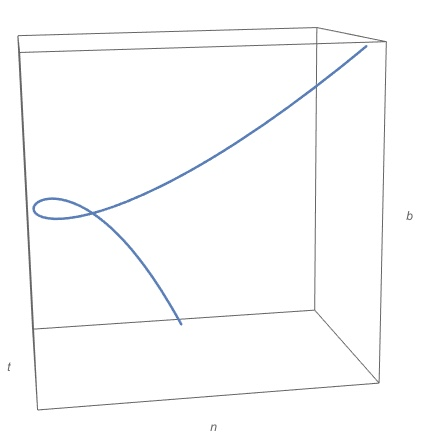
\includegraphics[scale=0.25]{figures_mvc/local_canonical_form}
	\end{center}
	\caption{Trace of a regular space curve in the neighborhood of a point with non-zero curvature and torsion.}
\end{figure}

\begin{figure}[h]
\centering
\begin{subfigure}{.5\textwidth}
  \centering
  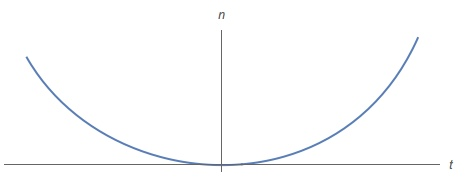
\includegraphics[width=.8\linewidth]{figures_mvc/tn_projection}
  \caption{Projection onto the osculating plane.}
  \label{fig:sub1}
\end{subfigure}%
\begin{subfigure}{.5\textwidth}
  \centering
  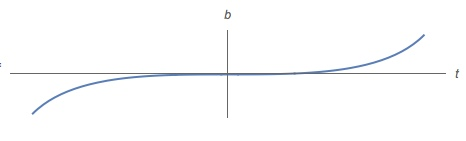
\includegraphics[width=.8\linewidth]{figures_mvc/tb_projection}
  \caption{Projection onto the rectifying plane.}
  \label{fig:sub2}
\end{subfigure}
\begin{subfigure}{.5\textwidth}
  \centering
  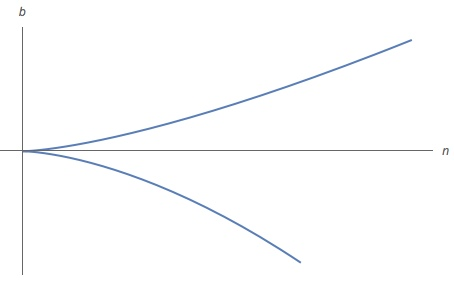
\includegraphics[width=.8\linewidth]{figures_mvc/bn_projection}
  \caption{Projection onto the normal plane.}
  \label{fig:sub3}
\end{subfigure}
\caption{Projections of a regular space curve in the neighborhood of a point with non-zero curvature and torsion onto the osculating, rectifying, and normal planes.}
\label{fig:test}
\end{figure}

Since $\kappa(s)>0$, the Taylor polynomial for $z(h)$ implies that if $\tau(s)>0$, then $z(h)>0$ for sufficiently small positive $h$. On the other hand, if $\tau(s)<0$, then $z(h)<0$ for sufficiently small positive $h$. Thus \emph{positive torsion} at $s$ implies that the the curve $\bbr$ is passing through the osculating plane at $s$ from below. Negative torsion implies from above. Here ``above" means the direction of $\ub(s)$.

\begin{figure}[h]
	\begin{center}
		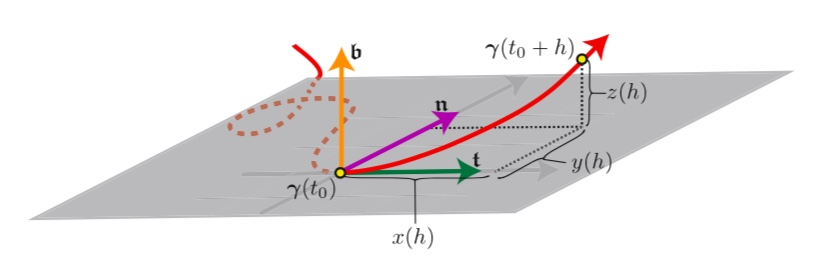
\includegraphics[scale=0.4]{figures_mvc/positive_torsion}
	\end{center}
	\caption{Positive torsion implies that the curve passes through the osculating plane from below.}
\end{figure}

To avoid taking the derivative of the cross product, here is another formula for the torsion which is often more computationally useful.

\begin{prop}
	Let $\bbr:I \to \mathbb{R}^3$ be a regular space curve with an arbitrary parametrization. Then for every $t \in I$ with $\kappa(t) \neq 0$, the torsion is given by
	\begin{align}\label{eq:torsion_jerk}
		\tau(t)=\frac{\bbr'(t) \times \bbr''(t)\cdot \bbr'''(t)}{||\bbr'(t) \times \bbr''(t)||^2}.
	\end{align}
In physical terms, the vector $\bbr'''(t)$ (the rate of change of acceleration) is called the \emph{jerk} at time $t$.
\end{prop}

\begin{proof}
	We will prove that this formula holds for a curve parametrized by arc length, and that it is also independent of parametrization, which then implies it holds for a curve with any parametrization.
	
	For a curve parametrized by arc length, $\bbr'(s)=\ut(s)$ and $\bbr''(s)=\kappa(s)\un(s)$, and therefore $\bbr'(s) \times \bbr''(s)=\kappa(s)(\ut(s) \times \un(s))=\kappa(s)\ub(s)$ and $||\bbr'(s) \times \bbr''(s)||=||\kappa(s)\ub(s)||=\kappa(s)$. Plugging into \eqref{eq:torsion_jerk}, we have
	\begin{align*}
		\tau(s)&=\frac{\ub(s) \cdot \bbr'''(s)}{\kappa(s)} \\
		&=\frac{\ub(s) \cdot (\kappa(s) \un(s))'}{\kappa(s)} \\
		&=\frac{\kappa'(s) \ub(s)\cdot \un(s)+\kappa(s)\ub(s)\cdot\un'(s)}{\kappa(s)} \\
		&=\frac{\kappa'(s) \cdot 0+\kappa(s)\ub(s)\cdot\un'(s)}{\kappa(s)} \\
		&=\ub(s) \cdot \un'(s) \\
		&=-\ub'(s) \cdot \un(s)
	\end{align*}
in agreement with Definition \ref{def:torsion_for_unit_speed_curve}.

To check that this formula is independent of parametrization, as we computed previously, if $\widetilde{\bbr}=\bbr \circ \varphi$, then
\begin{align*}
	\widetilde{\bbr}'(t)&=\varphi'(t)\bbr'(\varphi(t)) \\
	\widetilde{\bbr}''(t)&=\varphi''(t)\bbr'(\varphi(t))+(\varphi'(t))^2\bbr''(\varphi(t)) \\
	\widetilde{\bbr}'''(t)&=\varphi'''(t)\bbr'(\varphi(t))+3\varphi'(t)\varphi''(t)\bbr''(\varphi(t))+(\varphi'(t))^3\bbr'''(\varphi(t)).
\end{align*}
Then 
\begin{align*}
	\widetilde{\bbr}'(t)\times \widetilde{\bbr}''(t)&=\varphi'(t)\bbr'(\varphi(t))  \times [\varphi''(t)\bbr'(\varphi(t))+(\varphi'(t))^2\bbr''(\varphi(t))] \\
	&=\varphi'(t)\varphi''(t)\underbrace{\bbr'(\varphi(t))\times \bbr'(\varphi(t))}_{=0}+(\varphi'(t))^3(\bbr'(\varphi(t)) \times \bbr''(\varphi(t))) \\
	&=(\varphi'(t))^3(\bbr'(\varphi(t)) \times \bbr''(\varphi(t))) \\
\end{align*}
and therefore
\begin{align*}
	\widetilde{\tau}(t)&=\frac{(\varphi'(t))^3 (\bbr'(\varphi(t)) \times \bbr''(\varphi(t)))\cdot (\varphi'''(t)\bbr'(\varphi(t))+3\varphi'(t)\varphi''(t)\bbr''(\varphi(t))+(\varphi'(t))^3\bbr'''(\varphi(t)))}{(\varphi'(t))^6||\bbr'(\varphi(t)) \times \bbr''(\varphi(t))||^2}
\end{align*}
Using the cyclic property of the triple product \fixme{Refer to my Linear Algebra notes.}, we have 
\begin{align*}
	\bbr'(t) \times \bbr''(t) \cdot \bbr'(t)=\underbrace{\bbr'(t) \times \bbr'(t)}_{=0} \cdot \bbr''(t)  =0
\end{align*}
and 
\begin{align*}
	\bbr'(t) \times \bbr''(t) \cdot \bbr''(t) =\underbrace{\bbr''(t) \times \bbr''(t)}_{=0} \cdot \bbr'(t) =0
\end{align*}
so the formula becomes
\begin{align*}
	\widetilde{\tau}(t)&=\frac{(\varphi'(t))^6 (\bbr'(\varphi(t)) \times \bbr''(\varphi(t)))\cdot \bbr'''(\varphi(t)))}{(\varphi'(t))^6||\bbr'(\varphi(t)) \times \bbr''(\varphi(t))||^2}\\
	&=\frac{(\bbr'(\varphi(t)) \times \bbr''(\varphi(t)))\cdot \bbr'''(\varphi(t)))}{||\bbr'(\varphi(t)) \times \bbr''(\varphi(t))||^2} \\
	&=\tau(\varphi(t)) \\
\end{align*}
which shows $\tau$ is invariant under reparametrizations.
\end{proof}

\newpage 

\begin{example}
Consider the twisted cubic $\bbr(t)=(t,t^2,t^3)$ of Example	\ref{ex:twisted_cubic}. The unit binormal vector is given by 

\begin{figure}[h]
	\begin{center}
		\includegraphics[scale=0.5]{figures_mvc/tc_unit_binormal}
	\end{center}
\end{figure}

The torsion function is

\begin{figure}[h]
	\begin{center}
		\includegraphics[scale=0.5]{figures_mvc/tc_torsion_function}
	\end{center}
\end{figure}

Notice that the torsion takes its minimal value of 3 at $t=0$, and then strictly decreases as $|t| \to \infty$.
\end{example}

\subsection{Summary of formulas}
Let $\bv\equiv \bbr'$, $\ba\equiv \bbr''$, ${\bf j}\equiv \bbr'''$ and drop the dependence on the parameter $t$.
\subsubsection{Plane Curves}
\begin{enumerate}
	\item Unit tangent and unit normal vectors 
	\begin{align*}
		\ut=\frac{\bv}{||\bv||}, \hspace{0.5cm} \un = \frac{\ut'}{||\ut'||}
	\end{align*}
	\item Signed curvature function ($\bbr=(x,y)$)
	\begin{align*}
		\kappa_s=\frac{x'y''-x''y'}{((x')^2+(y')^2)^\frac{3}{2}}.
	\end{align*} 
	\item Curvature function ($\bbr=(x,y)$)
	\begin{align*}
		\kappa=|\kappa_s|=\frac{|x'y''-x''y'|}{((x')^2+(y')^2)^\frac{3}{2}}.
	\end{align*}
\end{enumerate}

\subsubsection{Space Curves}
\begin{enumerate}
	\item Frenet frame
	\begin{align*}
		\ut=\frac{\bv}{||\bv||}, \hspace{0.5cm} \un = \frac{\ut'}{||\ut'||}, \hspace{0.5cm} \ub=\ut \times \un.
	\end{align*}
	\item Curvature function
	\begin{align*}
		\kappa=\frac{||\bv \times \ba||}{||\bv||^3}.
	\end{align*}
	\item Torsion function
	\begin{align*}
		\tau=\frac{\bv \times \ba \cdot {\bf j}}{||\bv \times \ba||^2}.
	\end{align*}
\end{enumerate}

\appendix
\section{Proof of the Arc Length Formula}\label{app:arc_length}
\begin{prop}
The arc length formula 
\begin{align}
	s=\int_a^b||\bbr'(t)||dt.
\end{align}
can be obtained as the limit of a polygonal approximation of the curve.
\end{prop}

\begin{figure}[h]
	\begin{center}
	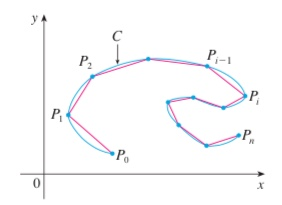
\includegraphics[scale=0.5]{figures_mvc/polygonal_approx}
\end{center}
\caption{A polygonal approximation of a regular curve.}
\end{figure}

\begin{pf}
\fixme{This proof references an idea here and there which are most likely unfamiliar. Attempts to give a rough explanation are given, but may not be entirely satisfactory.} Let $\bbr:I \to \R^n$ be a parametrized curve and let $[a,b] \subseteq I$. Let $a\equiv t_0<t_1<t_2	<\cdots<t_n\equiv b$ be a partition of $[a,b]$ where, for simplicity, we take each interval $t_i-t_{i-1}$ to have equal width $\Delta t\equiv \frac{b-a}{n}$. Approximate the length of curve between $\bbr(t_{i-1})$ and $\bbr(t_i)$ by a straight line. We then define the arc length $s$ between $\bbr(a)$ and $\bbr(b)$ by
\begin{align*}
	s&\equiv \lim_{n \to \infty}\sum_{i=1}^n||\bbr(t_i)-\bbr(t_{i-1})|| \\
	&=\equiv \lim_{n \to \infty}\sum_{i=1}^n\sqrt{(x(t_i)-x(t_{i-1}))^2+(y(t_i)-y(t_{i-1}))^2}.
\end{align*}
Since the coordinate functions $x(t)$ and $y(t)$ are continuous on $[a,b]$ and differentiable on $(a,b)$, by the Mean Value Theorem there exist $t_i^*$ and $t_i^{**}$ in $(a,b)$ such that
\begin{align*}
	x(t_i)-x(t_{i-1})&=x'(t_i^*)(t_i-t_{i-1}) \\
	&=x'(t_i^*)\Delta t \\
	y(t_i)-y(t_{i-1})&=y'(t_i^{**})(t_i-t_{i-1}) \\
	&=y'(t_i^{**})\Delta t
\end{align*}
and therefore
\begin{align*}
	s&=\lim_{n \to \infty}\sum_{i=1}^n\sqrt{(x'(t_i^*))^2+(y'(t_i^{**}))^2}\Delta t.
\end{align*}
If $t_i^*$ were equal to $t_i^{**}$ for all $i=1,\cdots,n$, then this would be a Riemann sum for $\int_a^b||\bbr'(t)||dt$. However, in general they are not equal, so we will instead show that the difference between this expression and the Riemann sum
\begin{align*}
\int_a^b||\bbr'(t)||dt\equiv\lim_{n \to \infty}\sum_{i=1}^n\sqrt{(x'(t_i^*))^2+(y'(t_i^*))^2}\Delta t	
\end{align*}
 goes to zero as $n \to \infty$. \footnote{Intuitively, this should make sense, since $t_i^*$ and $t_i^{**}$ both lie within $[t_{i-1},t_i]$ and by shrinking $\Delta t$, each of these subintervals also shrinks and therefore we should be able to make the points $t_i^*$ and $t_i^{**}$ become arbitrarily close to each other by making $\Delta t$ arbitrarily small.} First, note that since $\bbr$ is, in particular, continuously differentiable on each closed interval $[t_{i-1},t_i]$, the functions $x'$ and $y'$ are uniformly continuous on $[t_{i-1},t_i]$. \footnote{The proof of this involves the notion of ``compactness", the explanation of which would take us beyond the scope of this course. A function is said to be \emph{uniformly continuous} if for every $\epsilon>0$ there exists $\delta>0$ such that for any point $t \in [t_{i-1},t_i]$, $|t'-t|<\delta$ implies $||f(t)-f(t')||<\epsilon$; that is, the \emph{same} $\delta$ works for every point $t \in [t_{i-1},t_i]$. This is not true when a function is continuous but not uniformly continuous, since in that case $\delta$ depends on both $\epsilon$ \emph{and} $t$.} Thus, given any $\epsilon >0$ there exists a $\delta > 0$ such that $|t_i^*-t_i^{**}|< \delta$ implies $|y'(t_i^*)-y'(t_i^{**})|<\epsilon$. Since $|t_i^*-t_i^{**}|<t_i-t_{i-1}=\Delta t$, if we take $\Delta t < \delta$, then we will have $|y'(t_i^*)-y'(t_i^{**})|<\epsilon$. Note that this is possible since, given any $\delta > 0$, by the Archimedean property of the real numbers we can find a positive integer $n$ such that $\Delta t =\frac{b-a}{n}<\delta$. Assuming now that we have chosen $\Delta t<\delta$, we then have
\begin{align*}
	&\left|\sqrt{(x'(t_i^*))^2+(y'(t_i^{*}))^2}-\sqrt{(x'(t_i^*))^2+(y'(t_i^{**}))^2}\right|\\
	=& \left|\sqrt{(x'(t_i^*))^2+(y'(t_i^{*}))^2}-\sqrt{(x'(t_i^*))^2+(y'(t_i^{**}))^2+(y'(t_i^{*}))^2-(y'(t_i^{*}))^2}\right| \\
	=& \left|\sqrt{(x'(t_i^*))^2+(y'(t_i^{*}))^2}-\sqrt{(x'(t_i^*))^2+(y'(t_i^{*}))^2+(y'(t_i^{**}))^2-(y'(t_i^{*}))^2}\right|.
\end{align*}
Now $(y'(t_i^{**}))^2-(y'(t_i^{*}))^2 \leq |(y'(t_i^{**}))^2-(y'(t_i^{*}))^2|$, so, by the triangle inequality,
\begin{align*}
	\sqrt{(x'(t_i^*))^2+(y'(t_i^{*}))^2+(y'(t_i^{**}))^2-(y'(t_i^{*}))^2} &\leq \sqrt{(x'(t_i^*))^2+(y'(t_i^{*}))^2+|(y'(t_i^{**}))^2-(y'(t_i^{*}))^2|} \\
	&\leq \sqrt{(x'(t_i^*))^2+(y'(t_i^{*}))^2}+\sqrt{|(y'(t_i^{**}))^2-(y'(t_i^{*}))^2|} 
\end{align*}
and therefore
\begin{align*}
	&\left|\sqrt{(x'(t_i^*))^2+(y'(t_i^{*}))^2}-\sqrt{(x'(t_i^*))^2+(y'(t_i^{**}))^2}\right|\\
	=& \left|\sqrt{(x'(t_i^*))^2+(y'(t_i^{*}))^2}-\sqrt{(x'(t_i^*))^2+(y'(t_i^{*}))^2+(y'(t_i^{**}))^2-(y'(t_i^{*}))^2}\right| \\
	& \leq \left|\sqrt{(x'(t_i^*))^2+(y'(t_i^{*}))^2}-\left(\sqrt{(x'(t_i^*))^2+(y'(t_i^{*}))^2}+\sqrt{|(y'(t_i^{**}))^2-(y'(t_i^{*}))^2|}\right)\right| \\
	&=\left|-\sqrt{|(y'(t_i^{**}))^2-(y'(t_i^{*}))^2|}\right| \\
	&=\sqrt{|(y'(t_i^{**}))^2-(y'(t_i^{*}))^2|} \\
	&=\sqrt{|(y'(t_i^{**})+(y'(t_i^{*}))(y'(t_i^{**})-(y'(t_i^{*}))|} \\
	&=\sqrt{|(y'(t_i^{**})+(y'(t_i^{*}))|}\sqrt{|(y'(t_i^{**})-(y'(t_i^{*}))|} \\
\end{align*}
Since $y'$ is continuous and $[a,b]$ a closed interval, $y'([a,b])$ is bounded by some $M>0$, so \footnote{Here we have used the facts that the image of a compact set under a continuous mapping is compact, and that a compact set is bounded.}
\begin{align*}
	&=\sqrt{|(y'(t_i^{**})+(y'(t_i^{*}))|}\sqrt{|(y'(t_i^{**})-(y'(t_i^{*}))|} \\
	&\leq \sqrt{2M}\sqrt{|(y'(t_i^{**})-(y'(t_i^{*}))|},
\end{align*}
so by choosing $\Delta t<\delta$ such that $|(y'(t_i^{**})-(y'(t_i^{*}))|<\frac{\epsilon^2}{4M^2(b-a)^2}$, then 
\begin{align*}
	&\left|\sqrt{(x'(t_i^*))^2+(y'(t_i^{*}))^2}-\sqrt{(x'(t_i^*))^2+(y'(t_i^{**}))^2}\right|\\
	&\leq \sqrt{2M}\sqrt{|(y'(t_i^{**})-(y'(t_i^{*}))|} \\
	&< \sqrt{2M}\sqrt{\frac{\epsilon^2}{4M^2(b-a)^2}} \\
	&=\frac{\epsilon}{b-a}
\end{align*}
and therefore
\begin{align*}
	&\left|\sum_{i=1}^n\sqrt{(x'(t_i^*))^2+(y'(t_i^{*}))^2}\Delta t-\sum_{i=1}^n\sqrt{(x'(t_i^*))^2+(y'(t_i^{**}))^2}\Delta t\right| \\
	=&\left|\sum_{i=1}^n\left(\sqrt{(x'(t_i^*))^2+(y'(t_i^{*}))^2}-\sqrt{(x'(t_i^*))^2+(y'(t_i^{**}))^2}\right)\right|\Delta t \\
	&\leq \sum_{i=1}^n\left|\sqrt{(x'(t_i^*))^2+(y'(t_i^{*}))^2}-\sqrt{(x'(t_i^*))^2+(y'(t_i^{**}))^2}\right|\Delta t \\
	&<n\frac{\epsilon}{b-a} \Delta t \\
	&=n\frac{\epsilon}{b-a}\frac{(b-a)}{n} \\
	&=\epsilon.
\end{align*}
\end{pf}

\end{document}
